
\documentclass{article}
\usepackage{jim,amsmath}
\usepackage[utf8]{inputenc}
\usepackage[francais]{babel}
\usepackage[T1]{fontenc}

\usepackage{xcolor,graphicx}
\usepackage{comment}
\usepackage{verbatim}
\usepackage{balance}


\newenvironment{gmncode}	{\vspace{-2mm}\small\verbatim}{\endverbatim\vspace{-2mm}}
%\newenvironment{code}  		{\fontfamily{pnc}\selectfont}{}

\newcommand{\guido}			{\textsc{Guido}}
\newcommand{\gmn}			{\textsc{gmn}}
\newcommand{\code}[1]		{{\small \texttt{#1}}}
\newcommand{\guidotag}[1]	{\textbackslash\code{#1}}
\newcommand{\exemple}		{\vspace{2mm}\hspace*{-6mm}\textsc{Exemple}}

\title{\centering Extension de Guido aux notations contemporaines}

%\date{ Février - décembre 2013}

\oneauthor
 {Camille Le Roi, Colas Decron, Dominique Fober} {
 Grame - Centre national de création musicale \\ 
\{cleroi, decron, fober\}@grame.fr
 }

%\threeauthors
%  {Camille Le Roi} {Grame \\ cleroi@grame.fr}
%  {Colas Decron} 	{Grame \\ cdecron@grame.fr}
%  {Dominique Fober} {Grame \\ fober@grame.fr}

\begin{document}

\selectlanguage{french}

\maketitle

\begin{abstract}

Le projet \guido{} regroupe à la fois un format textuel de description de partitions musicales, un moteur de rendu basé sur ce format, et une librairie qui fournit aux développeurs d'applications, un support de haut niveau pour l'ensemble des services liés au format \guido{} et à son rendu sous forme graphique. 
De base, le projet \guido{} traite de la notation traditionnelle de la musique occidentale. Le projet a été récemment étendu, tant du point de vue format que du point de vue rendu, pour adresser également les besoins les plus courants de la musique contemporaine. Cet article présente ces extensions et montre comment les choix de design fournissent à l'utilisateur une large palette de solutions pour la notation de la musique. 

%La librairie \guido{} offre un grand nombre de symboles musicaux correspondant aux plus larges besoins de l'écriture musicale. Elle fournit un moteur de rendu de partitions embarquable dans d'autres applications. Dans une volonté d'étendre cette librairie à la musique contemporaine, nous avons implémenté un ensemble de nouvelles notations jusqu'à présent pas, ou très sommairement, implémentées. L'objectif était de répondre aux demandes des compositeurs en ajoutant certaines notations de la manière la plus adaptée à l'écriture musicale, tout en laissant une large liberté à l'utilisateur.

\end{abstract}

%%%%%%%%%%%%%%%%%%% INTRODUCTION %%%%%%%%%%%%%%%%%%%%

\section{Introduction}\label{sec:introduction}

% format
% librairie
% compos
% état de l'art de la notation contemporaine
% pb de la notation contemporaine
% 
% Studying Music is Difficult and Important, Donald Byrd
% Music Notation Software and Intelligence, Donald Byrd
% A Brief Survey of Music Representation Issues Techniques and Systems
% Les logiciels d'aide à la composition musicale


Le projet \guido{} est né il y a presque 20 ans, tout d'abord comme format textuel de représentation de la musique \cite{hoos98,guido}, puis comme moteur de rendu graphique de partitions musicales \cite{RENZ02}. 
Lors de sa conception, le format \guido{} se différencie des approches proposées par SCORE \cite{SCORE}, MuseData \cite{Hewlett97}, DARMS \cite{darms} ou encore Humdrum \cite{Huron97} notamment parce qu'il est pleinement lisible par l'utilisateur. Basée sur un formalisme qui aborde la description de la musique à partir des concepts musicaux, l'approche développée par \guido{} repose sur l'idée d'adéquation, qui invite à noter simplement les concepts musicaux simples, et à ne recourir à des notations complexes que pour les notions musicales complexes.

Postérieurement au format \guido{}, d'autres représentations textuelles de la notation de la musique ont vu le jour, telles que Lilypond \cite{lilypond03,lilypond06} qui est assez similaire dans son format, ou MusicXML \cite{good01}, orienté vers l'échange de partitions. Toutefois, le projet \guido{} reste unique parce qu'il est le seul qui propose à la fois un format de notation, une moteur de rendu et une librairie C/C++ permettant d'embarquer des capacités de rendu de partitions dans des applications indépendantes.
Par ailleurs, la rapidité et l'efficacité du moteur de rendu le rendent utilisable dans un contexte \textit{temps réel} (pour des partitions dont le niveau de complexité n'est pas trop élevé), ouvrant la voie à des formes d'interactivité inédites \cite{Hoadley12,Fober:12a}.

Pour répondre aux besoins les plus courants de la musique contemporaine, le format \guido{} ainsi que le moteur de rendu ont étés étendus. Après un bref rappel sur le format \guido{}, cet article décrit ces extensions en  situant les choix qui ont été faits en terme de rendu graphique, dans les pratiques identifiées dans la littérature contemporaine. Nous montrerons également comment une forme de \emph{langage générique} permet de combiner ces représentations et offre à l'utilisateur un large éventail de solutions pour la représentation de la musique.


%Le format de notation musicale \guido{} (GMN) \cite{hoos98} \cite{Dau:09a} a été défini par H. Hoos et K. Hamel il y a plus de 10 ans. Il est très proche du format adopté par Lilypond \cite{lilypond03,lilypond06} mais il est apparu antérieurement. Le format GMN est un langage textuel de représentation de partitions musicales 
%. Il est basé sur un formalisme simple mais puissant, se concentrant sur les grands concepts musicaux (en opposition aux caractéristiques graphiques). L'approche développée par \guido{} repose sur l'idée d'adéquation, qui invite à noter simplement les concepts musicaux simples, et à ne recourir à des notations complexes que pour les notions musicales complexes.
%sur lequel est basée %sur le format GMN, 
%la librairie \guido{} \cite{Dau:09a}. Cette dernière %fournit un puissant moteur de mise en page de partitions, qui 
%se différencie notamment des approches de type compilateur par sa capacité à être embarquée dans une application indépendante, et par la rapidité et l'efficacité du moteur de rendu, qui le rendent utilisable dans un contexte temps réel pour des partitions simples.


%%%%%%%%%%%%%%%%%%%%% FORMAT GMN %%%%%%%%%%%%%%%%%%
\section{Le format de Notation Guido}\label{sec:format_notation}

Ci-dessous figurent les principes généraux du format de notation \guido{}. Ils sont fournis pour permettre la compréhension du contenu des sections suivantes. Pour plus de détails on peut se reporter à \cite{Dau:09a} ou \cite{guido}.

Le format de base de \guido{} recouvre les notes, silences, altérations, voix indépendantes, et les concepts les plus courants de la notation musicale comme les clefs, métriques, armures, articulations, liaisons, etc.
Les notes sont représentées par leur nom \code{(a b c d e f g h)}, une altération optionnelle (\code{\#} et \code{\&} pour dièse et bémol), un numéro d'octave optionnel et une durée optionnelle exprimée sous forme de fraction.

%Le format de base de \guido{} recouvre les notes, silences, altérations, voix indépendantes, et les concepts les plus courants de la notation musicale comme les clefs, métriques, armures, articulations, liaisons, etc.
%Les notes sont représentées par leur nom, une altération optionnelle, un numéro d’octave optionnel et une durée optionnelle. Les accords sont décrits par des notes entre accolades séparées par des virgules. Un système (d'une ou plusieurs portées) est décrit par deux accolades, et une portée par deux crochets.


Les \emph{tags} sont utilisés pour donner des informations musicales supplémentaires, comme les liaisons, clés, armures, etc. Un \emph{tag} a une des formes suivantes : 
\begin{gmncode}
    \tagname<param-list>
    \tagname<param-list>(note-series)
\end{gmncode}
%\begin{code}
%\textbackslash{}tagname<param-list>
%\textbackslash{}tagname\textless{}param-list\textgreater{}(note-series)
%\end{code}
où \emph{param-list} est une liste optionnelle de paramètres (chaînes de caractères ou nombres), et où \emph{note-series} est l'ensemble des notes ou accords concernés par le \emph{tag}. Dans ce cas nous parlerons de \emph{range-tag} (\emph{tag} possédant une durée explicite).


%%%%%%%%%%%%%%%%%%%%%%% NOUVEAUTES %%%%%%%%%%%%%%%%%%%
\section{Extensions de la notation}\label{sec:extension}

%**************************** MICRO TONALITES *****************************
\subsection{Micro-tonalité}\label{subsec:micro}

La micro-tonalité a été introduite avec la version 1.43 de la librairie \guido{}. Graphiquement, elle est limitée à la représentation du quart de ton alors que d'un point de vue langage, elle s'exprime comme un nombre flottant de demis tons, qui sont arrondis au quart de ton le plus proche pour le rendu graphique: 
\begin{gmncode}
    1)  \alter<detune>
    2)  \alter<detune>(note-series)
\end{gmncode}

La première forme (1) introduit la notion d'\emph{altération courante} : l'altération reste valide jusqu'à une indication contraire. Dans la deuxième forme (2), l'altération ne s'applique qu'aux notes indiquées.

\exemple\\
Le code suivant produit le résultat présenté en figure \ref{fig:alter}.
\begin{gmncode}
[
  a&& \alter<-1.5>(a) a& \alter<-0.5>(a)  
  a \alter<0.5>(a) a# \alter<1.5>(a) 
  \alter<1.8>(a)
]
\end{gmncode}

\begin{figure}[h]
\centering
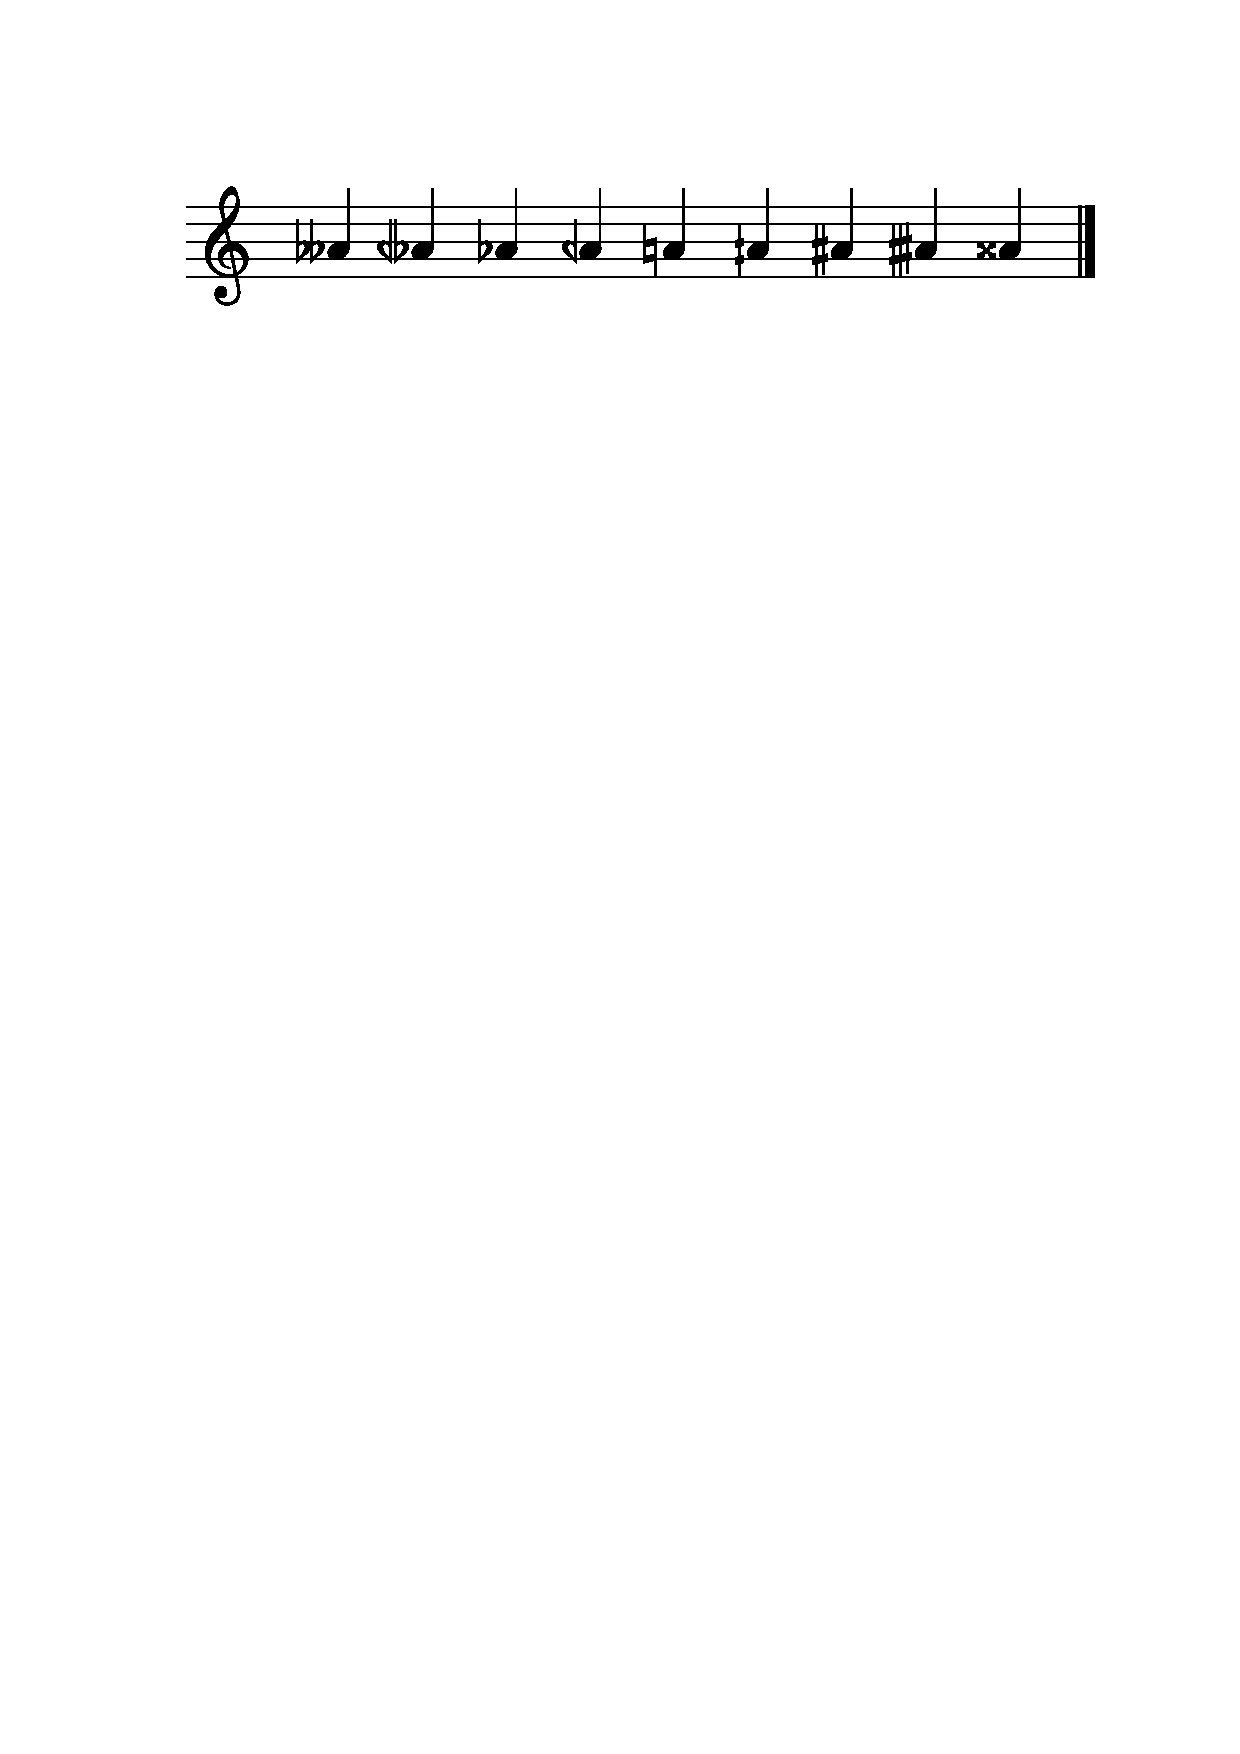
\includegraphics[width=\columnwidth]{img/partitions/alter.pdf}
\caption{Micro-tonalité}
\label{fig:alter}
\end{figure}

La micro-tonalité est également introduite dans les armures de clef libres. De manière similaire, elle s'exprime sous forme de nombres flottants indiqués entre crochets.

\exemple
\begin{gmncode}
[
  \key<"free=c[1.5]g#b&a[-1.5]"> a g# 
  \alter<0.5> g  a \alter<1.5> g 
]
\end{gmncode}
Le résultat est présenté en figure \ref{fig:freekey}.
\begin{figure}[h]
\centering
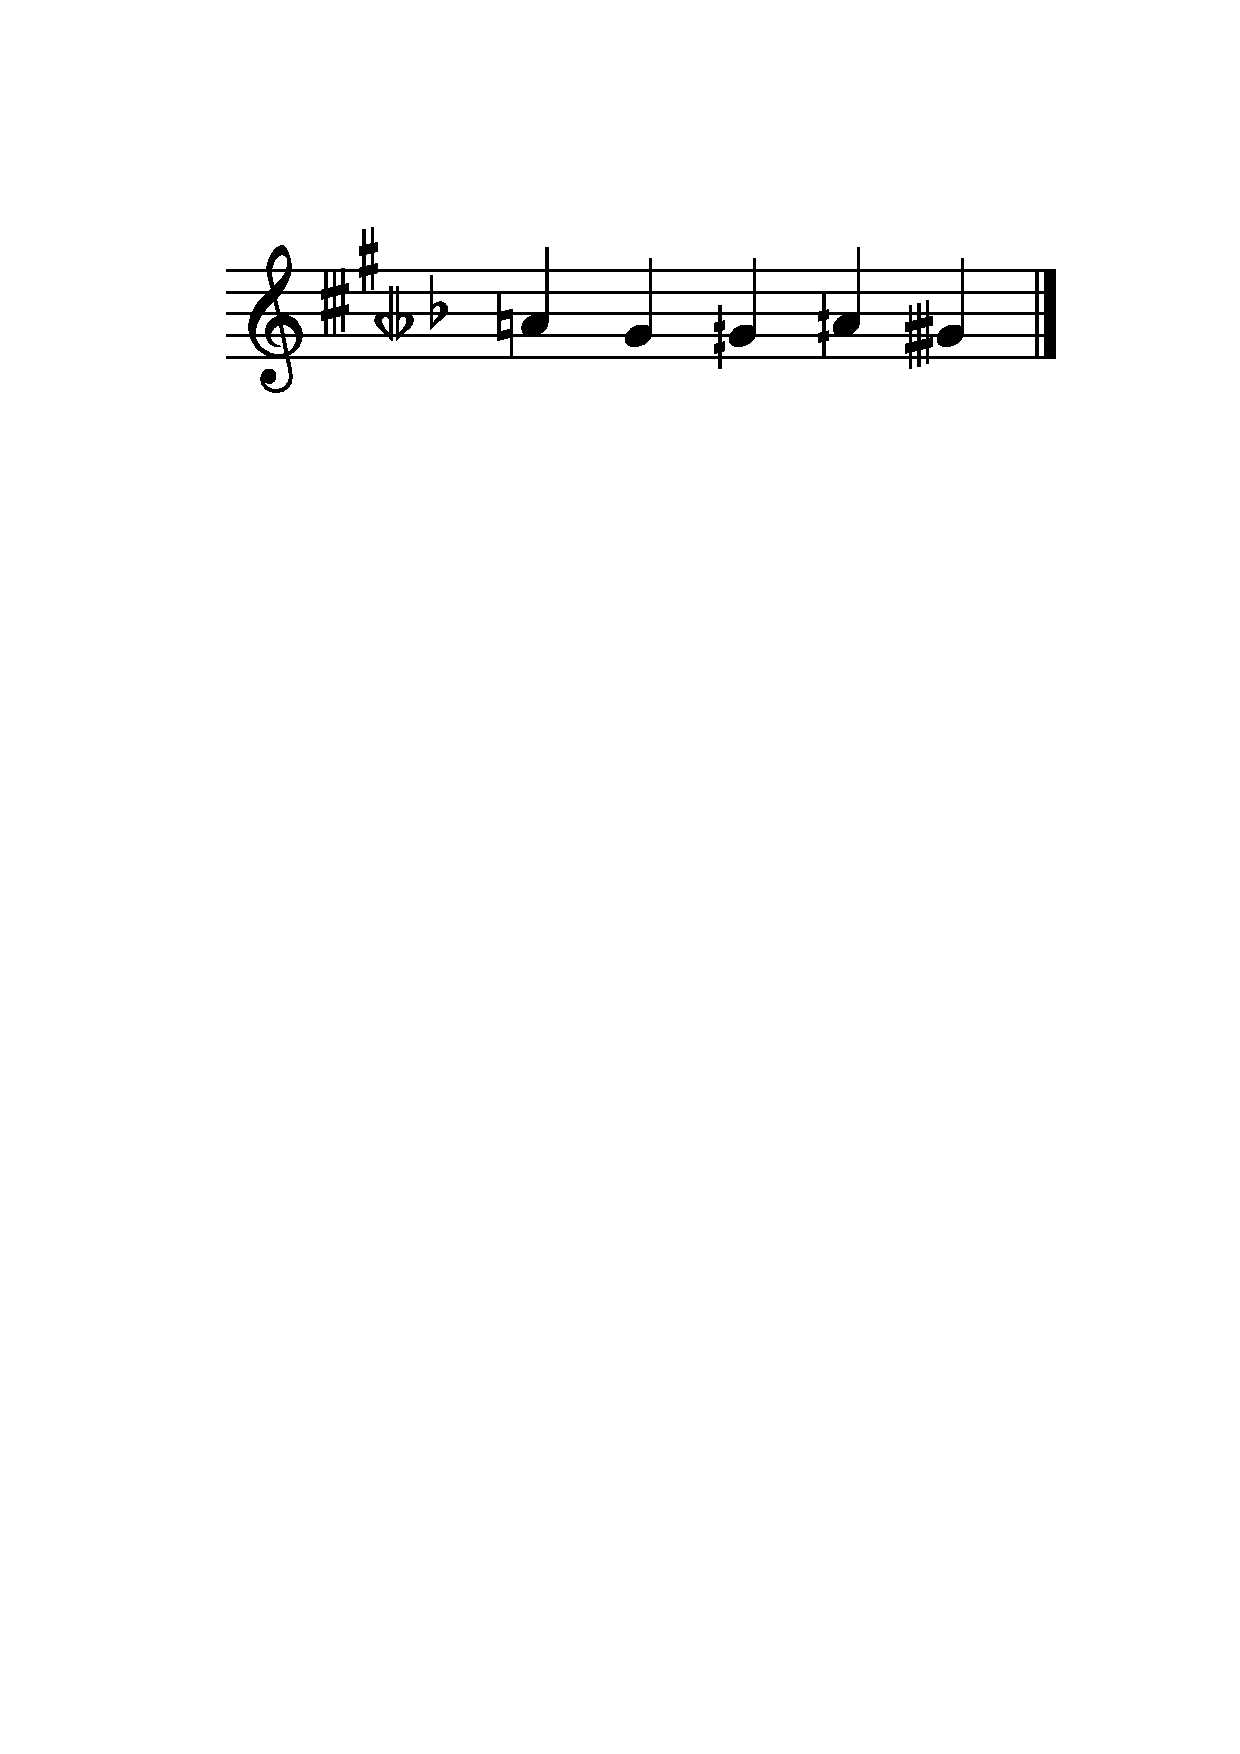
\includegraphics[width=0.75\columnwidth]{img/partitions/freekey.pdf}
\caption{Armure de clef libre avec micro-tonalité}
\label{fig:freekey}
\end{figure}


%**********************TETES DE NOTES *****************************
\subsection{Têtes de notes}\label{subsec:tetes_notes}
%
La librairie \guido{} a été étendue avec 6 nouveaux symboles de têtes de note qui sont spécifiés par le paramètre \code{style} du tag \guidotag{noteFormat}:
\begin{gmncode}
  \noteFormat<style=noteHeadStyle>
\end{gmncode}
où \code{noteHeadStyle} est parmi :
\begin{itemize}
    \item \code{x} : une croix
    \item \code{diamond} : un diamant
    \item \code{round} : un rond
    \item \code{square} : un carré
    \item \code{triangle} : un triangle, pointe en haut
    \item \code{reversedTriangle} : un triangle, pointe en bas
\end{itemize} 

\vspace{2mm}
La première portée de l'exemple de la figure \ref{fig:noteheads} est générée avec le code suivant:
\begin{gmncode}
[
  \noteFormat<style="x"> a
  \noteFormat<style="diamond"> a
  \noteFormat<style="round"> a
  \noteFormat<style="square"> a
  \noteFormat<style="triangle"> a
  \noteFormat<style="reversedTriangle"> a
]
\end{gmncode}
%
\begin{figure}[h]
\centering
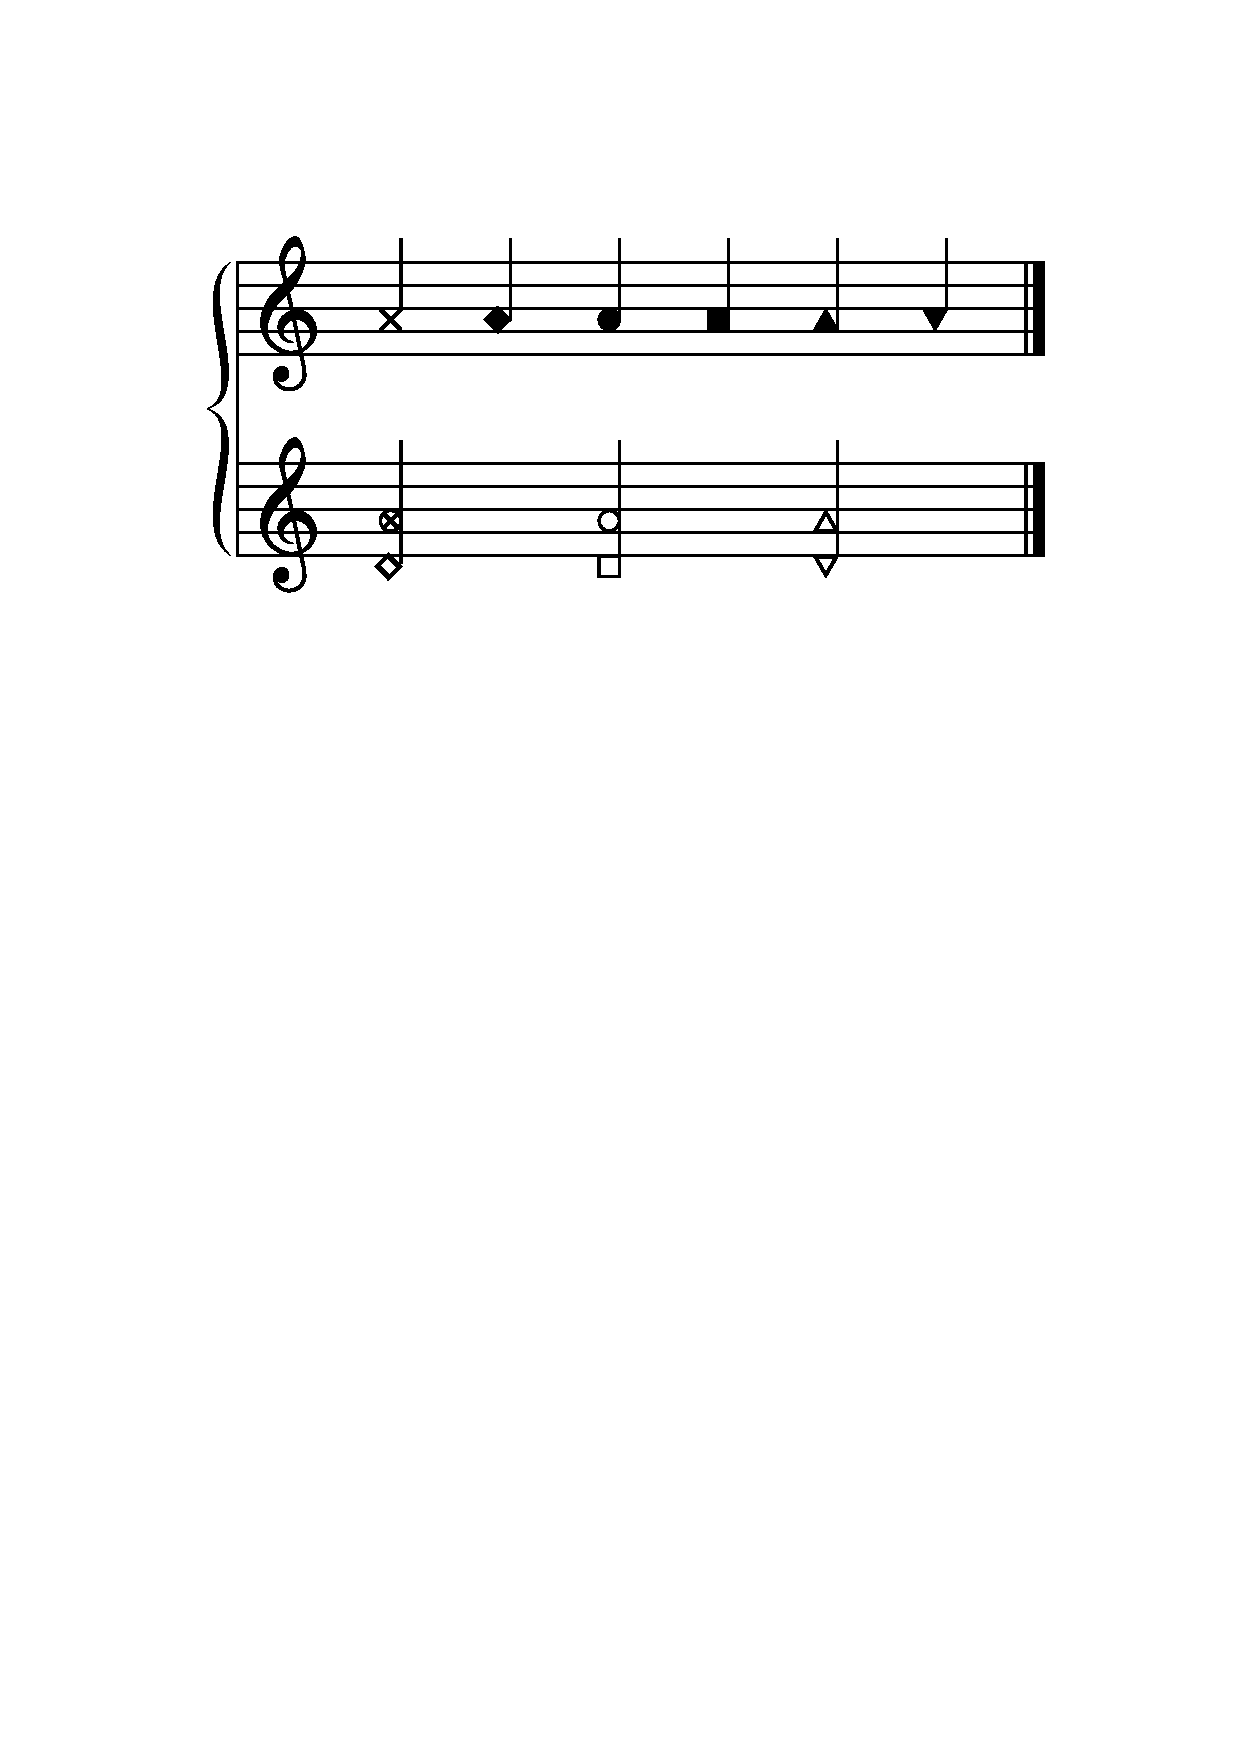
\includegraphics[width=6cm]{img/partitions/noteheads.pdf}
\caption{Les 6 nouveaux \emph{noteheads} ajoutés}
\label{fig:noteheads}
\end{figure}
%
Pour l'apparence graphique de ces éléments, nous nous sommes principalement inspirés des ouvrages de E. Gould \cite{gould2011behind} et de K. Stone \cite{stone1980music}.
L'implémentation repose sur le tag \guidotag{noteFormat} déjà existant, qui modifie l'apparence des notes qui le suivent (couleur, taille, offset, etc.). Nous avons rajouté un attribut de \code{style}, permettant à l'utilisateur de choisir l'apparence des têtes de notes.

Des ajustements graphiques particuliers ont été nécessaires pour tenir compte des différences graphiques entre les têtes de notes :
\begin{itemize}
    \item insertion d'un offset horizontal variable selon le symbole choisi, l'orientation de la hampe, l'utilisation en accord ou non (les accords pouvant posséder des têtes de notes différentes pour chacune de leurs notes);
    \item adaptation de la longueur de la hampe selon le type symbole utilisé (par exemple, différence de longueur entre le \code{triangle} et le \code{reversedTriangle}).
\end{itemize}


%**************************** COMPLEX METER ********************************
\subsection{Métriques complexes}\label{subsec:metriques}

% Pourquoi le texte n'est pas justifié ?
La possibilité d'insérer une métrique complexe a été introduite avec la version 1.52 de la librairie \guido{}. Elle permet d'indiquer une subdivision de la métrique par une somme en place et lieu de la métrique habituelle. La syntaxe est la même que pour une métrique normale, elle fait usage du tag \guidotag{meter} et il suffit de remplacer le numérateur par une somme, comme le montre l'exemple ci-dessous, illustré en figure \ref{fig:complexMeter}.

\exemple\\
\begin{gmncode}
  [ \meter<"3+3+2/4"> a b g ]
\end{gmncode}

\begin{figure}[h]
\centering
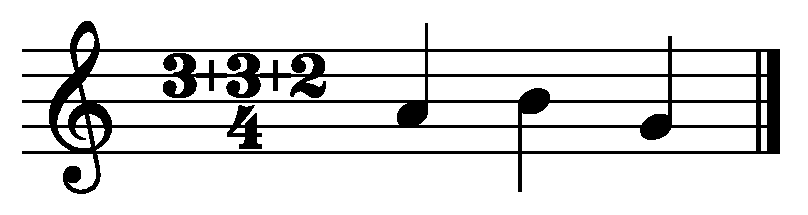
\includegraphics[width=50mm]{img/partitions/complexMeter.pdf}
\caption{Métrique complexe}
\label{fig:complexMeter}
\end{figure}

%**************************** CLUSTERS ********************************
\subsection{\emph{Clusters}}\label{subsec:clusters}

Un \emph{cluster} est un accord musical contenant plusieurs notes consécutives. Il peut par exemple être effectué sur un piano, où il se joue en déclenchant des touches contiguës (en utilisant son avant-bras, par exemple).

Un \emph{cluster} est indiqué par un range-tag s'appliquant à des accords de deux notes: les notes extrêmes du \emph{cluster} (les autres notes éventuelles seront ignorées) :

\begin{gmncode}
\cluster<param-list>(chord-series)
\end{gmncode}

\begin{figure}[h]
\centering
\begin{gmncode}
[
  \cluster({a, d} {c/8, f}
    {a/2, d2} {f/1, c1})
]
\end{gmncode}
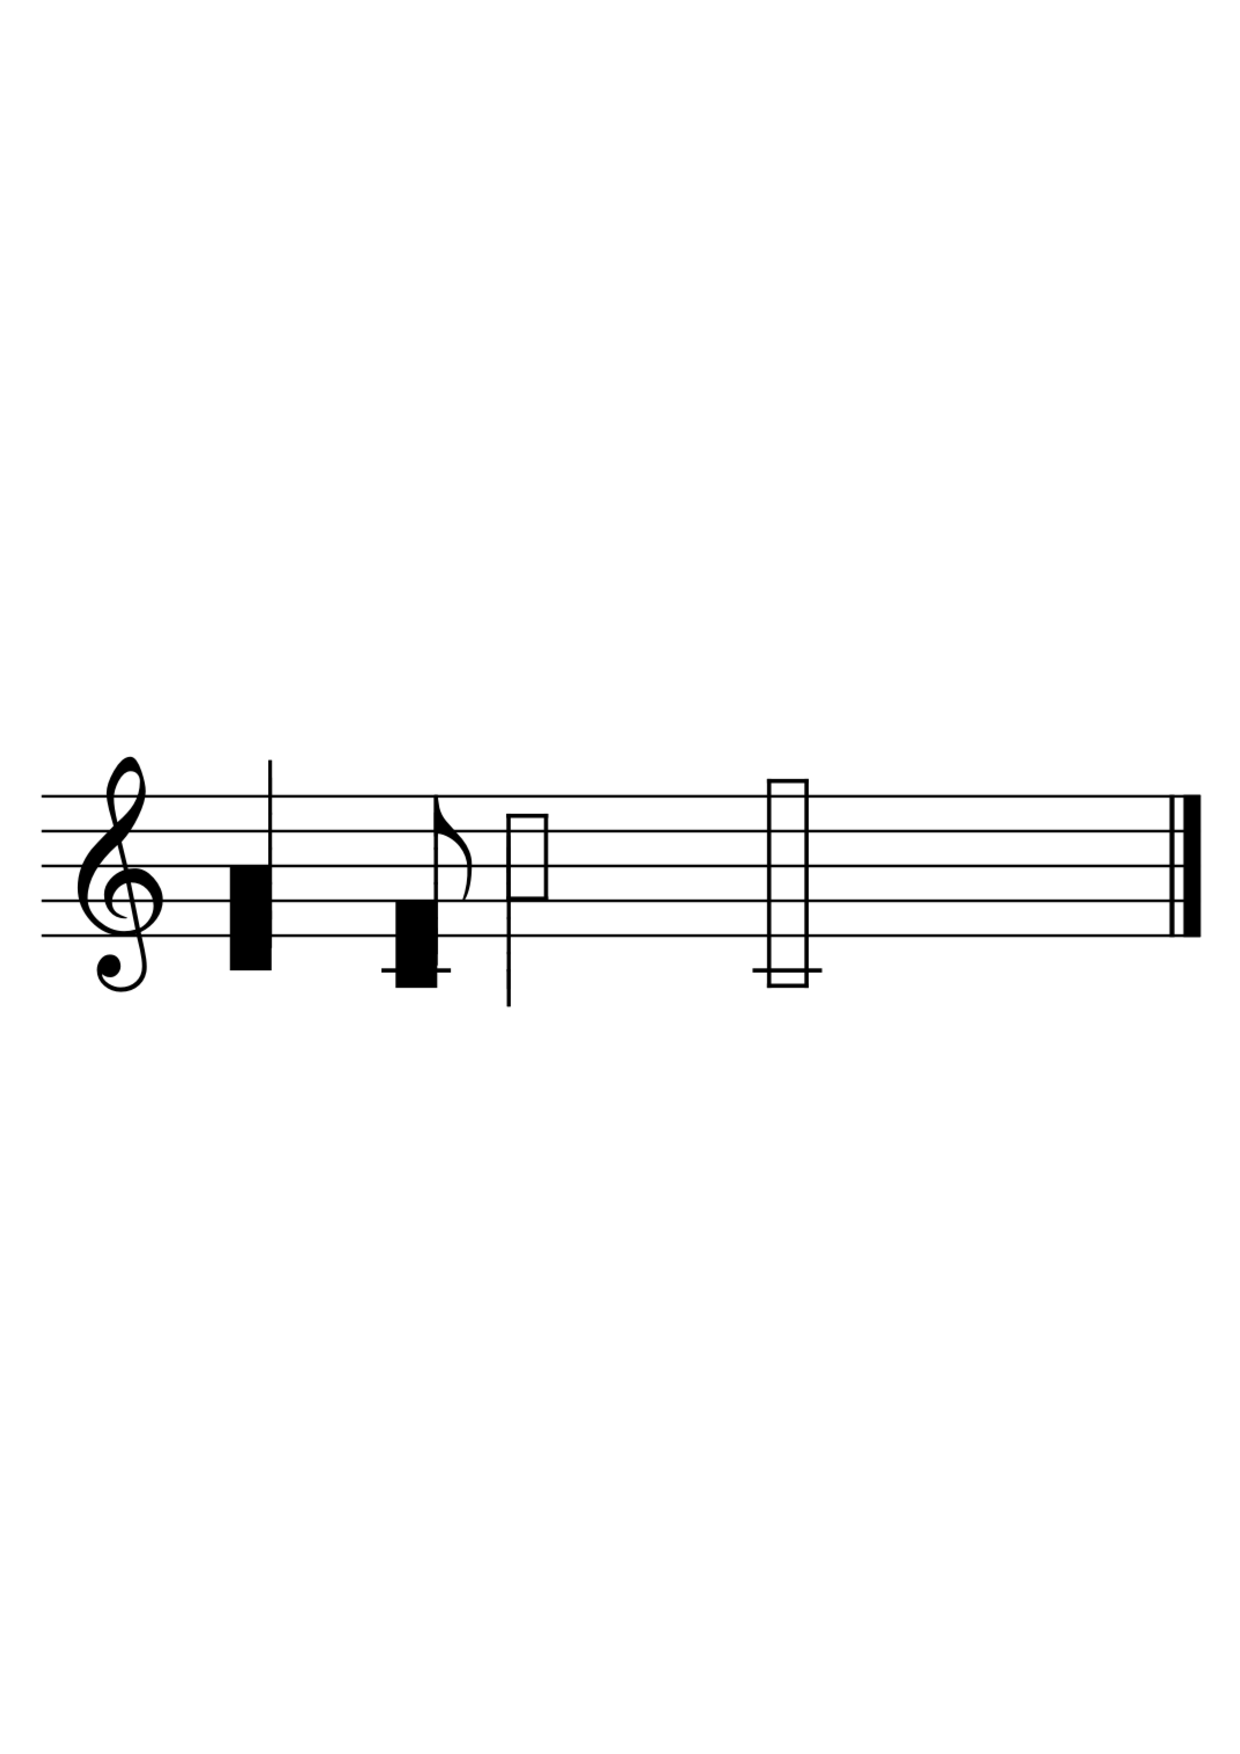
\includegraphics[width=50mm]{img/partitions/cluster.pdf}
\caption{\emph{Cluster}}
\label{fig:cluster}
\end{figure}
%

Comme l'indique en partie la figure \ref{fig:cluster}, les choix, faits à partir d'ouvrages référents \cite{gould2011behind,stone1980music} ont été les suivants:
\begin{itemize}
	\item le \emph{cluster} est représenté par un rectangle;
	\item ce rectangle est plein ou vide, selon la durée du \emph{cluster};
	\item la hampe est conservée pour garder l'indication de la durée.
\end{itemize}

Le tag \guidotag{cluster} supporte les paramètres de contrôle standard (\code{size}, \code{dx}, \code{dy}, \code{color}) auxquels ont été ajoutés des paramètres \code{hdx} et \code{hdy} permettant d'introduire un décalage s'appliquant à la tête de note. 

Un cluster est vu comme une note et supporte donc le tag \guidotag{noteFormat} ainsi que le contrôle de l'orientation des têtes de notes (\guidotag{headsReverse}, \guidotag{headsLeft} et \guidotag{headsRight}) ainsi qu'illustré en figure \ref{fig:clusterInteractions}).

\exemple
\begin{figure}[h]
\centering
\begin{gmncode}
[
  \cluster<color="red", hdx=1, hdy=3>({a})
  \cluster<size=0.5>({f,c2})
  \noteFormat<color="purple">
  \headsReverse
  \cluster<color="green", size=2>({f, g2})
  \cluster<"blue">({d1/2, g})
]
\end{gmncode}
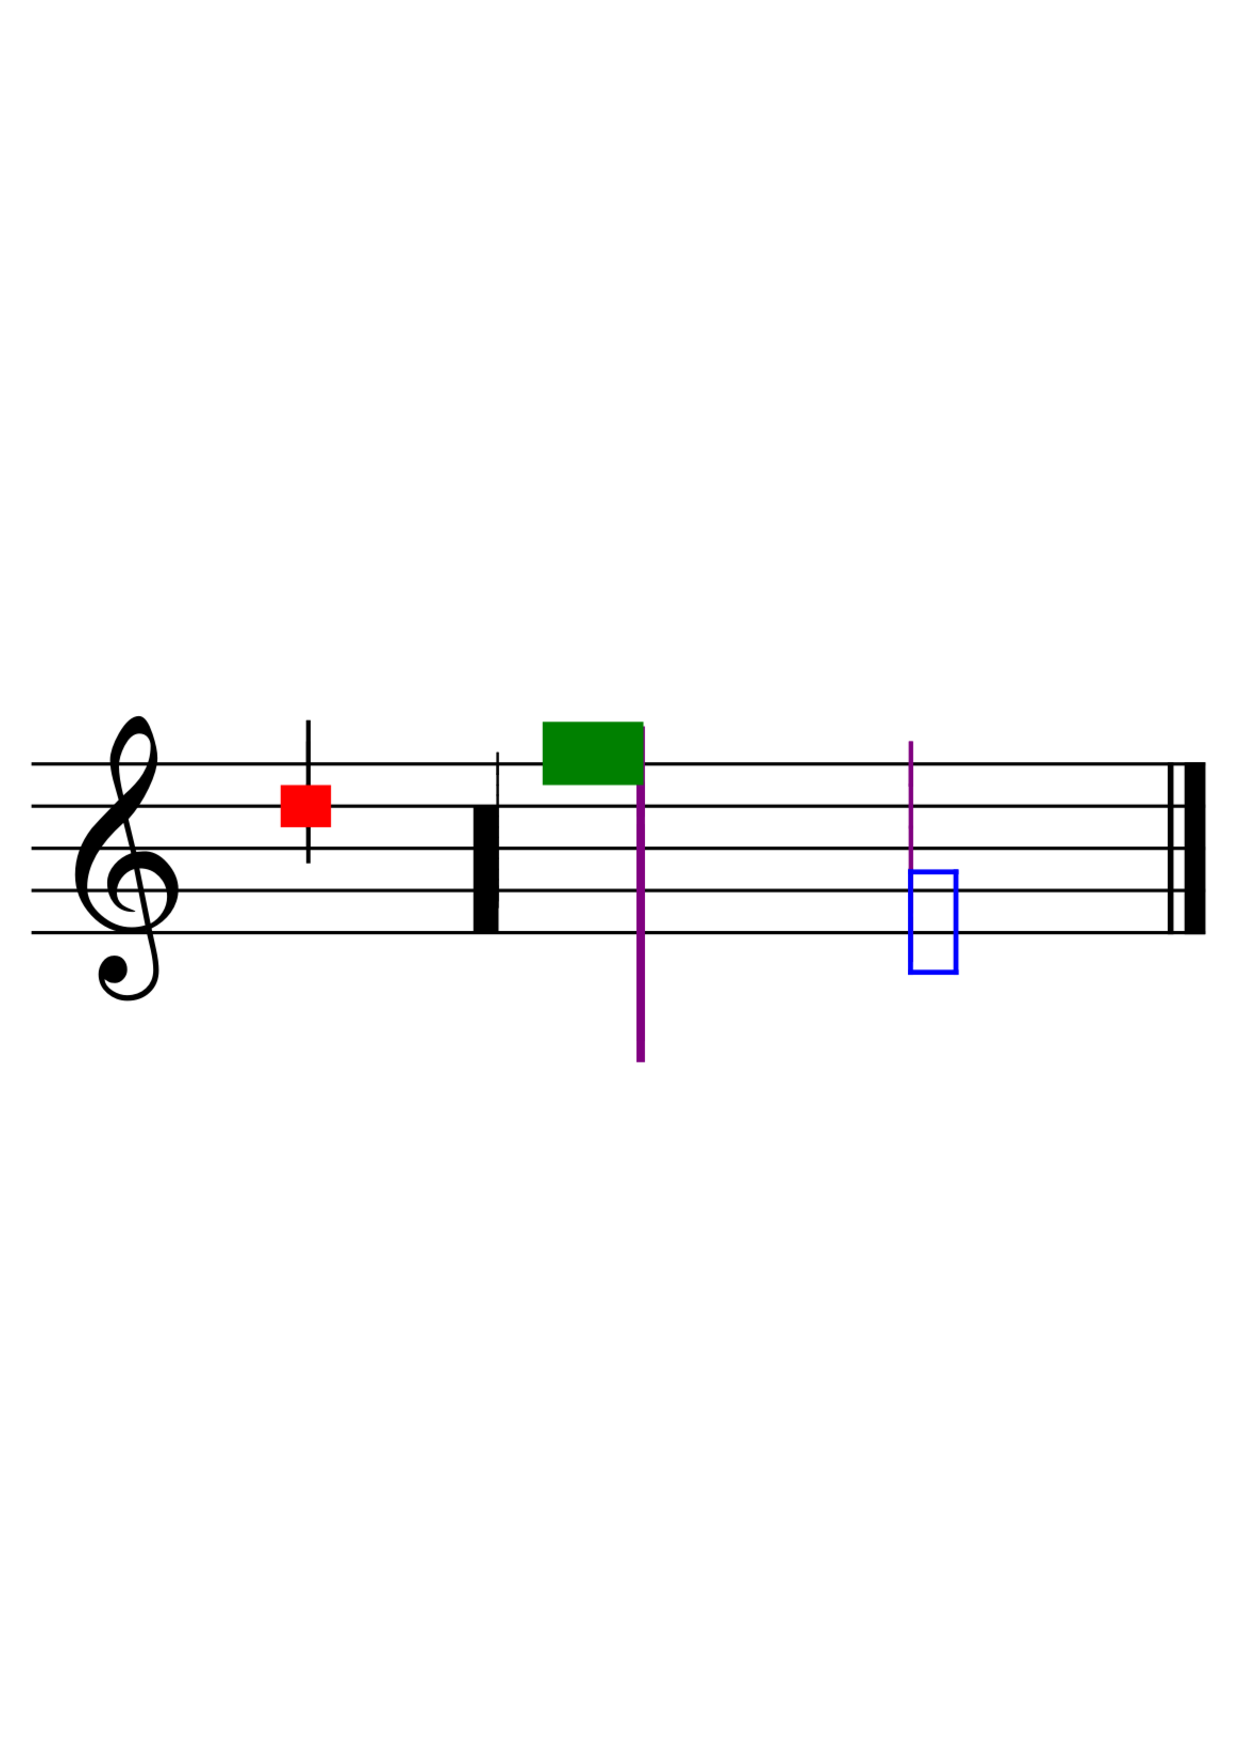
\includegraphics[width=45mm]{img/partitions/clusterInteractions.pdf}
\caption{Les interactions avec d'autres tags}
\label{fig:clusterInteractions}
\end{figure}
%


%***************GLISSANDO************************
\subsection{Glissando}\label{subsec:glissando}

Le \emph{glissando} se présente classiquement comme une ligne joignant deux notes décalées dans le temps ( Figure \ref{fig:glissandoSimple} ), indiquant ainsi un glissement, continu ou non suivant le type d'instrument, d'une hauteur à l'autre.

Dans un souci d'efficacité, il fallait pouvoir décrire un \emph{glissando} seul ou plusieurs \emph{glissandi} à la suite de la manière la plus simple et intuitive possible. 

\begin{gmncode}
  \glissando<params>( notes )
  params : 
    - fill = "true" ou "false": 
      option de remplissage
    - thickness = float : 
      épaisseur de la ligne
\end{gmncode}

Il paraissait important de donner la possibilité à l'utilisateur de n'écrire qu'une seule fois le tag pour décrire plusieurs \emph{glissandi} consécutifs, contrairement à la description de lilypond où le tag doit être répété entre chaque note. Ainsi le range-tag apparaissait comme la meilleure solution pour décrire un ou plusieurs \emph{glissandi} : toutes les notes comprises dans les parenthèses seraient prises en compte et liées les unes aux autres par des \emph{glissandi}. L'algorithme de démultiplication d'un même tag et de répartition de celui-ci est fortement inspiré de celui du \guidotag{tie}, ou liaison de prolongation, qui doit également créer une liaison entre chacune des notes affectées.


\exemple
\begin{figure}[h]
\centering

\begin{gmncode}
  [ \glissando( g b d ) ]
\end{gmncode}

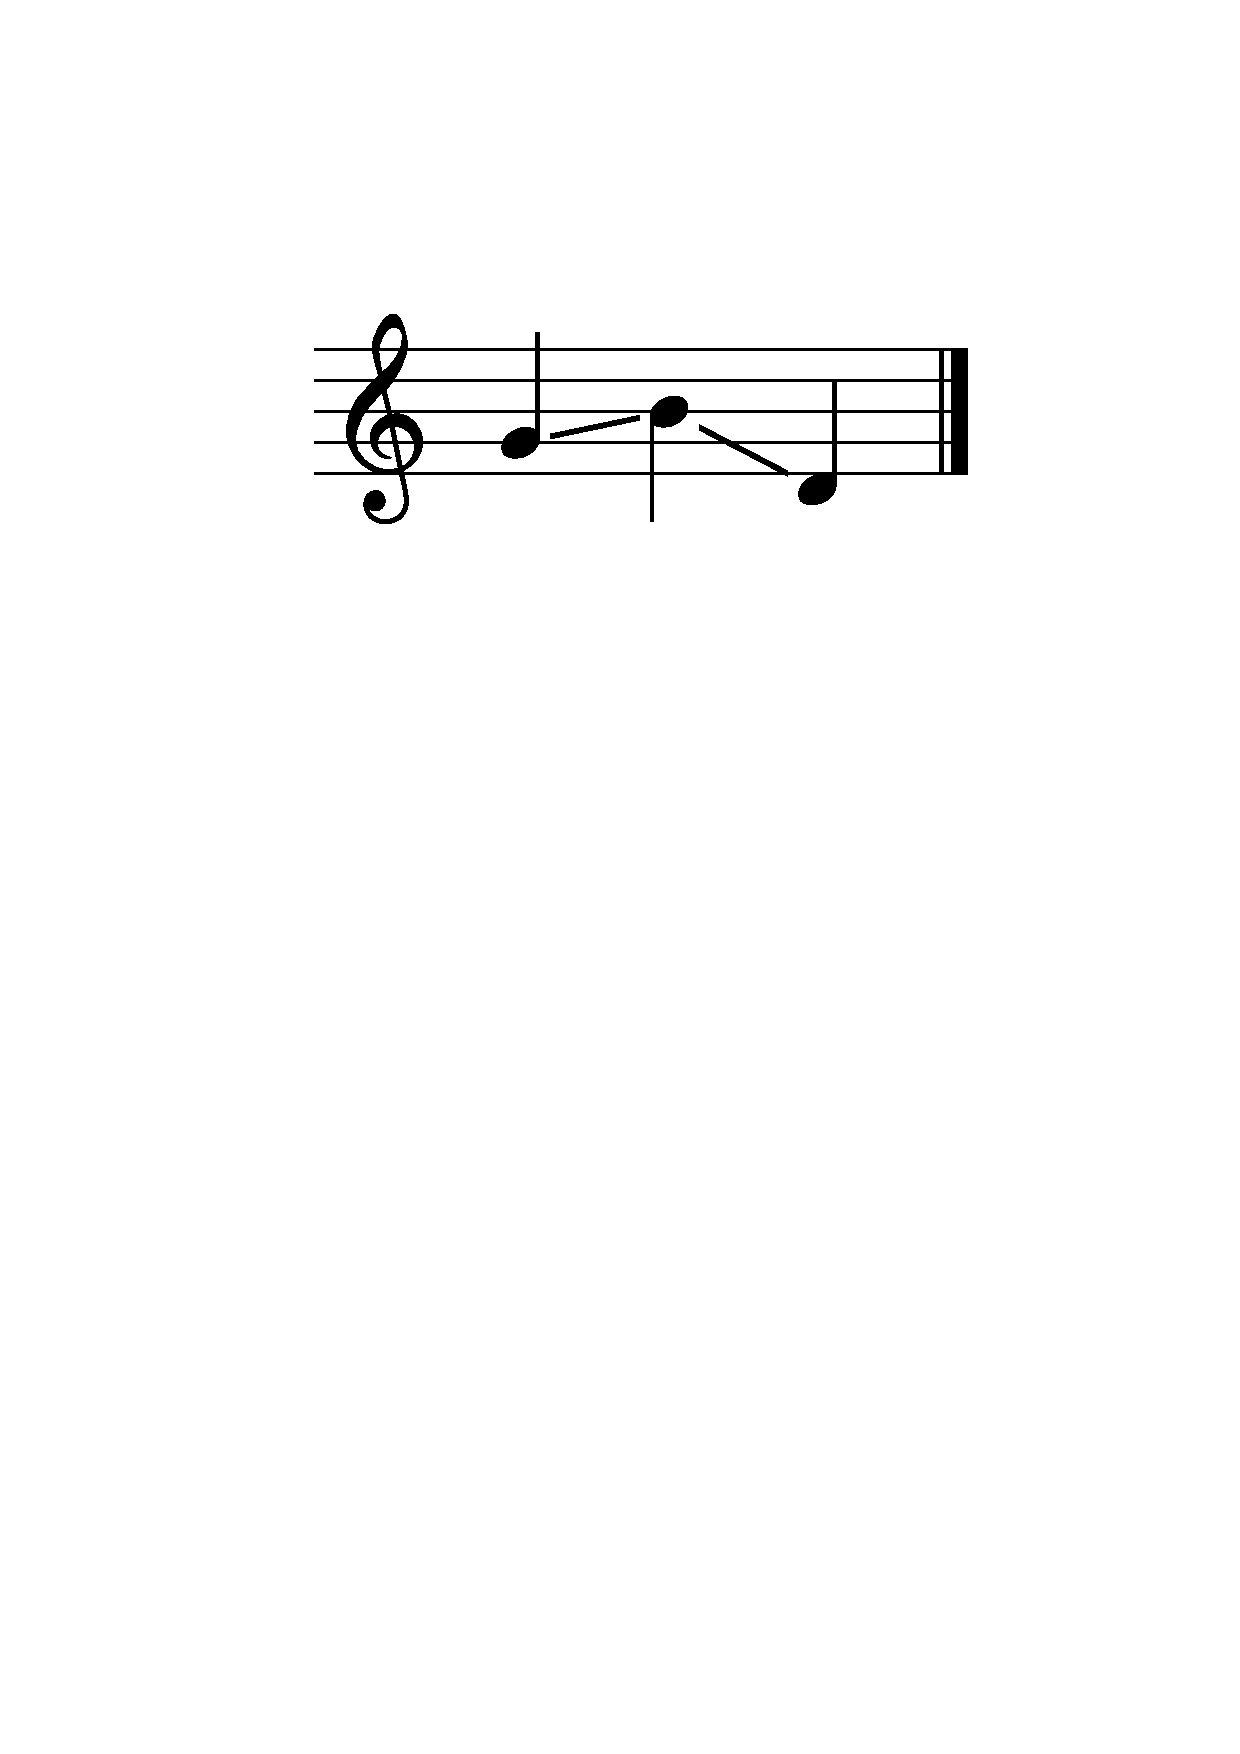
\includegraphics[width=35mm]{img/glissando1.pdf}
\caption{\emph{Glissando}}
\label{fig:glissandoSimple}
\end{figure}




% *********************** FEATHERED BEAM ****************************
\subsection{Liens de croches en soufflet (\emph{feathered beaming})}\label{subsec:featheredBeaming}
\bigskip

\begin{gmncode}
  \fBeam<params>( notes )
  params : 
    - durations="firstDur, lastDur" : 
      durée des première et dernière notes
    - drawDuration : 
      indication de la durée totale
\end{gmncode}

Décrite par Gardner Read comme "a highly graphic representation of rythmic flexibility"  \cite{read1969music} (p.94), cette notation contemporaine d'un accelerando ou ritardando à travers les liens de croches est, de manière générale, encore peu répandue dans les ouvrages de théorie, et se résume souvent à des cas simples, partant ou arrivant à la simple croche, c'est à dire partant de, ou arrivant vers, un unique point. Pourtant il paraît intéressant de pouvoir offrir la possiblité aux compositeurs de décrire le passage entre n'importe quelles valeurs : par exemple d'une double-croche à une triple-croche, ou d'une quadruple-croche à une double-croche... (Figure \ref{fig:fbeamcomplex})

\exemple
\begin{figure}[h]
\centering
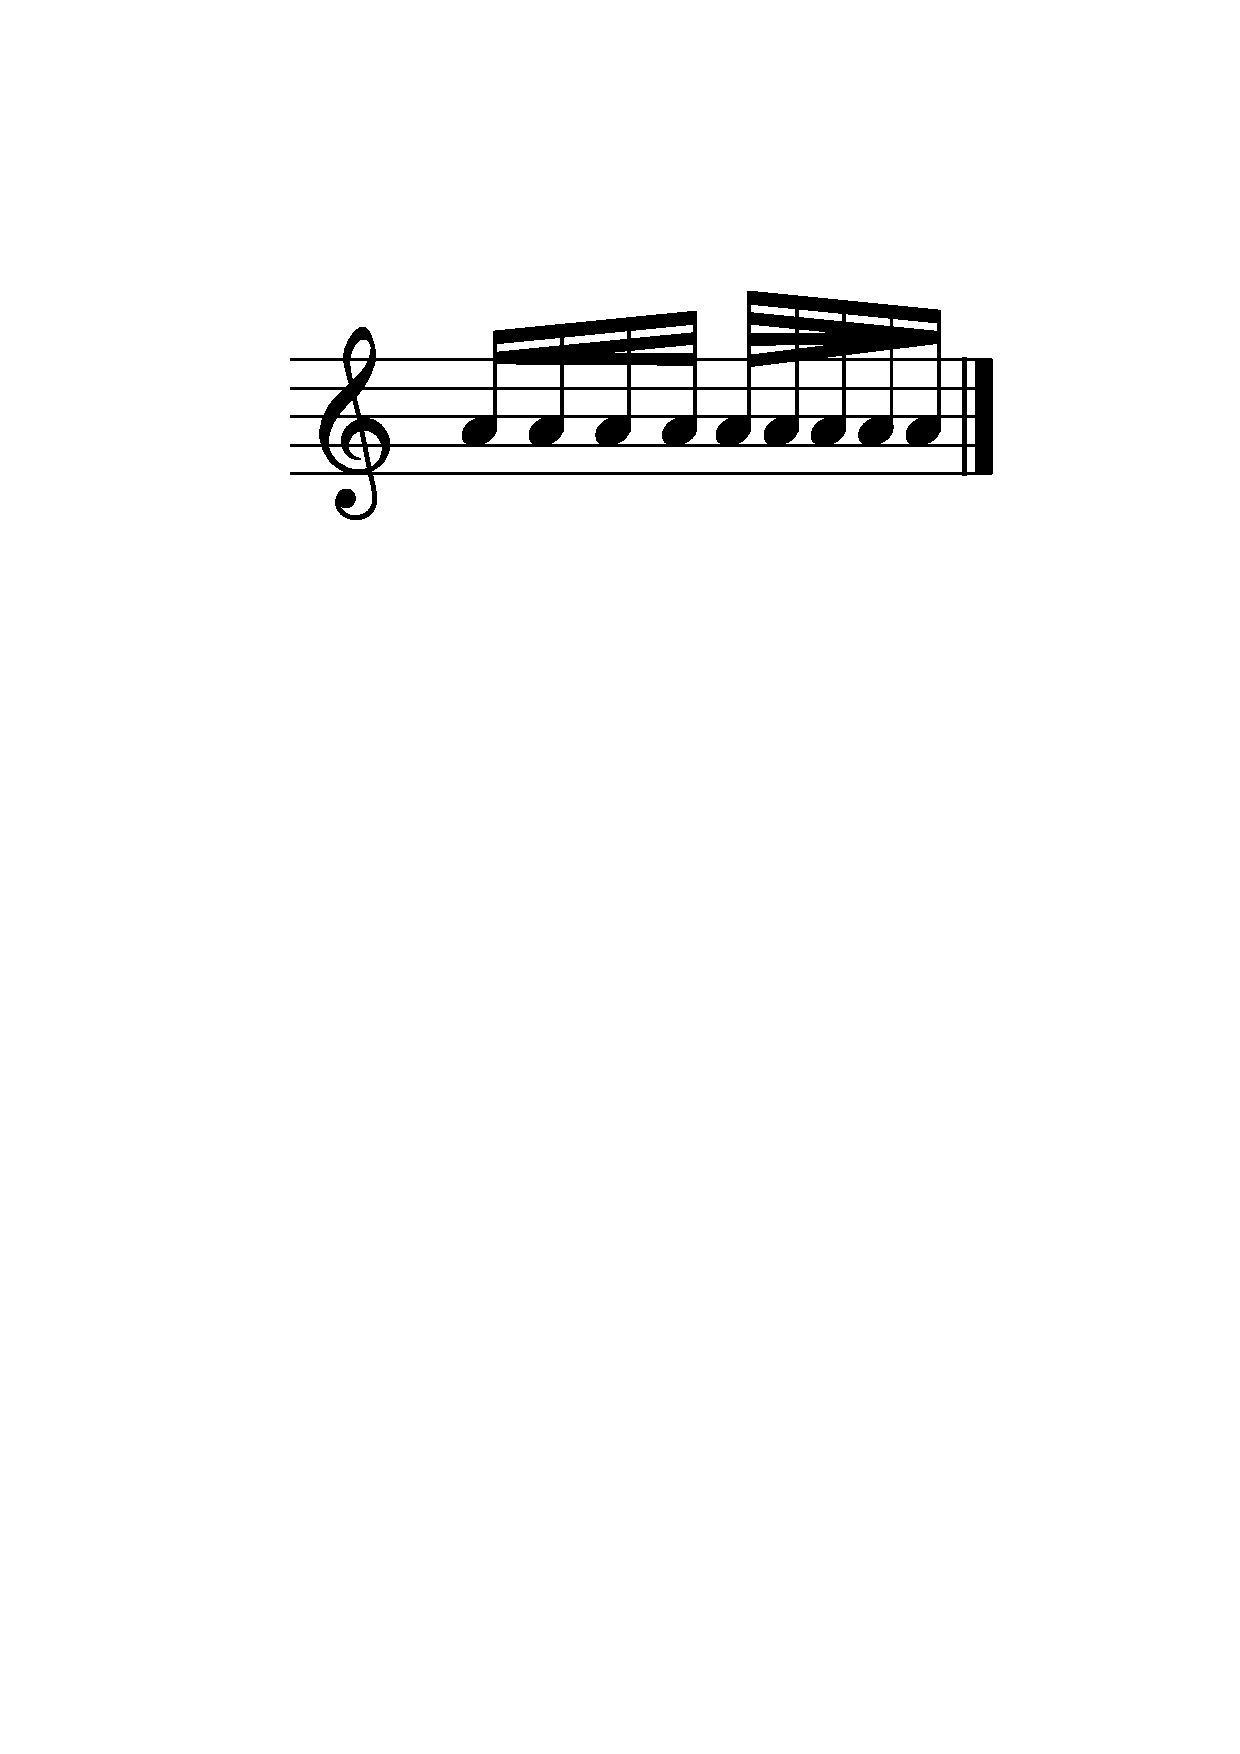
\includegraphics[width=40mm]{img/fbeamcomplex.pdf}
\caption{\emph{feathered beams} plus complexes}
\label{fig:fbeamcomplex}
\end{figure}

Dans un désir de simplicité, il a été décidé de décrire par un seul range-tag un seul groupe de notes liées, correspondant à un point de départ et un point d'arrivée uniques.

Il est cependant possible de chaîner plusieurs \emph{feathered beams} en utilisant la forme \code{Begin / End} des range-tag (i.e \guidotag{fBeamBegin} et \guidotag{fBeamEnd}), permettant alors, non seulement de chaîner deux \emph{beams} par une note (Figure \ref{fig:fbeamchain}), mais aussi de les faire se chevaucher sur plusieurs notes.

\begin{figure}[h]
\exemple
\begin{gmncode}
[ 
  \fBeamBegin:1 c/8 d e/16 
  \fBeamBegin:2 f/32 \fBeamEnd:1 
  e/16 d/8 c \fBeamEnd:2 
]
\end{gmncode}

\begin{center}
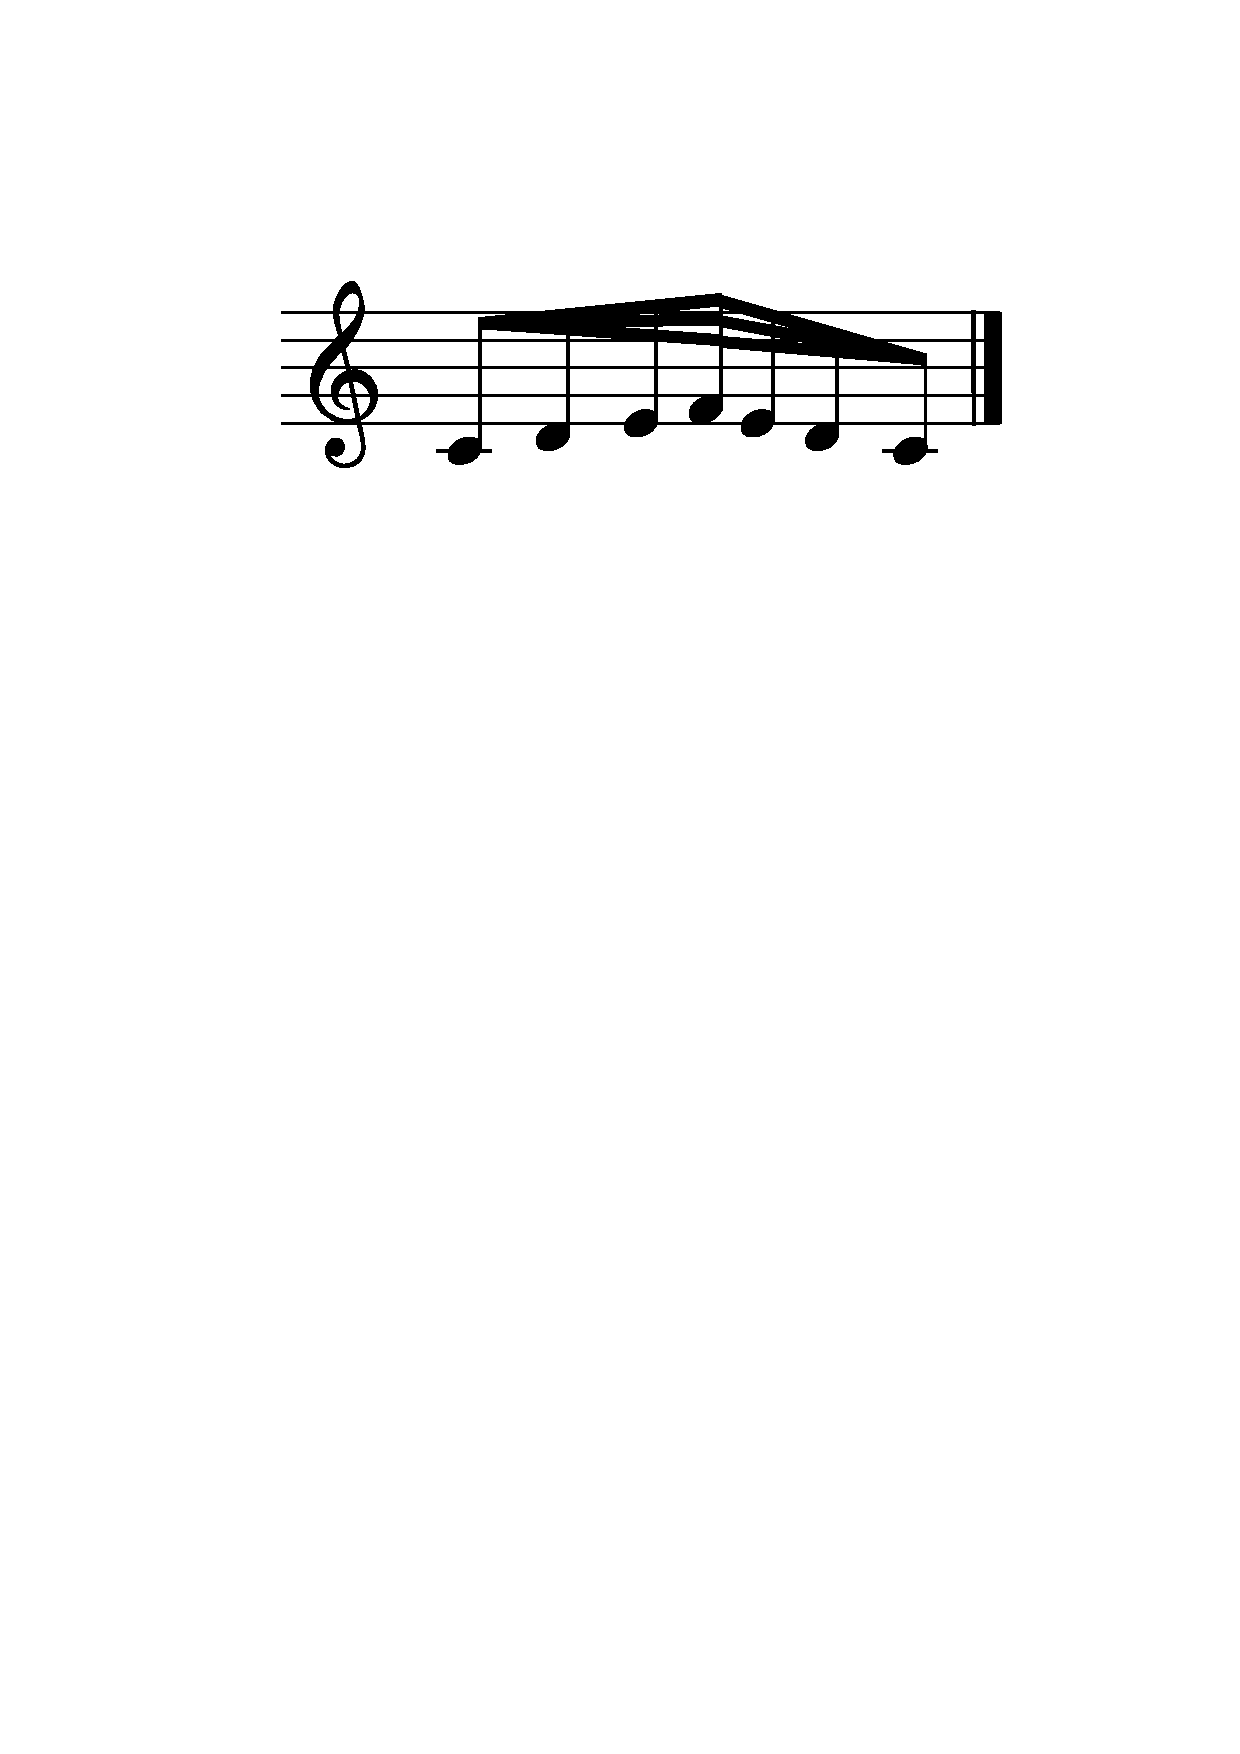
\includegraphics[width=45mm]{img/fBeamChaine.pdf}
\end{center}
\caption{\emph{Feathered beams} chaînés}
\label{fig:fbeamchain}
\end{figure}

% question de voix simultanées
% lilypond : 
% \override Beam #'grow-direction = #LEFT
% \featherDurations #(ly:make-moment 2 1)
% { c16[ c c c c c c c] }
\bigskip
On remarque que, même dans un ouvrage tel que celui d'Elaine Gould \cite{gould2011behind}, peu de détails sont donnés sur cette notation, et on se heurte rapidement à des incohérences telles que celle de la figure \ref{fig:incoherence} tirée de "Behind Bars" : on veut faire tenir en un temps une croche et quatre notes de durées inférieures à la croche mais supérieures à la triple-croche. 

\begin{figure}[h]
\centering
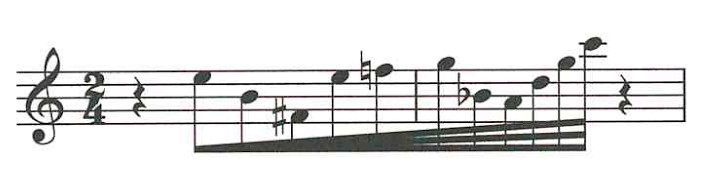
\includegraphics[width=8cm]{img/behindbars.jpg}
\caption{Exemple d'incohérence entre la durée totale et les durées individuelles des notes d'un groupe lié. (Behind Bars, p.158) }
\label{fig:incoherence}
\end{figure}

Ce manque d'une exacte cohérence entre tempo et aspect graphique est également souligné par Kurt Stone \cite{stone1980music} : "Besides, the gradual increase or decrease in the number of beams makes exact indications of beat-units impossible" (p.124).

Ainsi on voit l'importance des choix de design de ce symbole, sur la manière de le décrire textuellement, de le dessiner en particulier dans le cas de plusieurs voix simultanées, et de manière générale sur la liberté laissée à l'utilisateur.
\\

Concernant les possibilités de description données à l'utilisateur. Nous avons vu que plusieurs critères pouvaient intervenir dans la description, et devaient pouvoir être imposés par l'utilisateur. Des paramètres qui peuvent être incohérents entre eux :
\begin{itemize}
\item le nombre de notes dans le groupe,
\item leurs durées individuelles et intrinsèques qui définissent également leur espacement,
\item la durée totale du groupe, dépendante directement des durées individuelles,
\item les durées de départ et d'arrivée qui définissent l'aspect graphique du \emph{feathered beam}.
\end{itemize}
\bigskip

Ces différents niveaux de description nous poussent à faire une claire distinction entre l'aspect temporel et l'aspect graphique de notre groupe de notes.  Il a été décidé de laisser au compositeur la liberté de donner à son \emph{feathered beam} l'aspect graphique qu'il désire, indépendamment des durées internes de ses notes. Il pourra ainsi jouer sur les espacements entre notes, sur le nombre de notes, et sur la durée totale de manière "classique" en imposant à chaque note une durée, et en veillant à ce que la somme de toutes les notes corresponde à la durée totale souhaitée. Cette durée totale peut être indiquée sur la partition grâce au paramètre \code{drawDuration} (Figure \ref{fig:fbeamduree}).

\exemple
\begin{figure}[h]
\centering
\begin{gmncode}
[ 
  \fBeam<drawDuration="true">
  ( a/8 a a/16 a a a/32 a ) 
]
\end{gmncode}
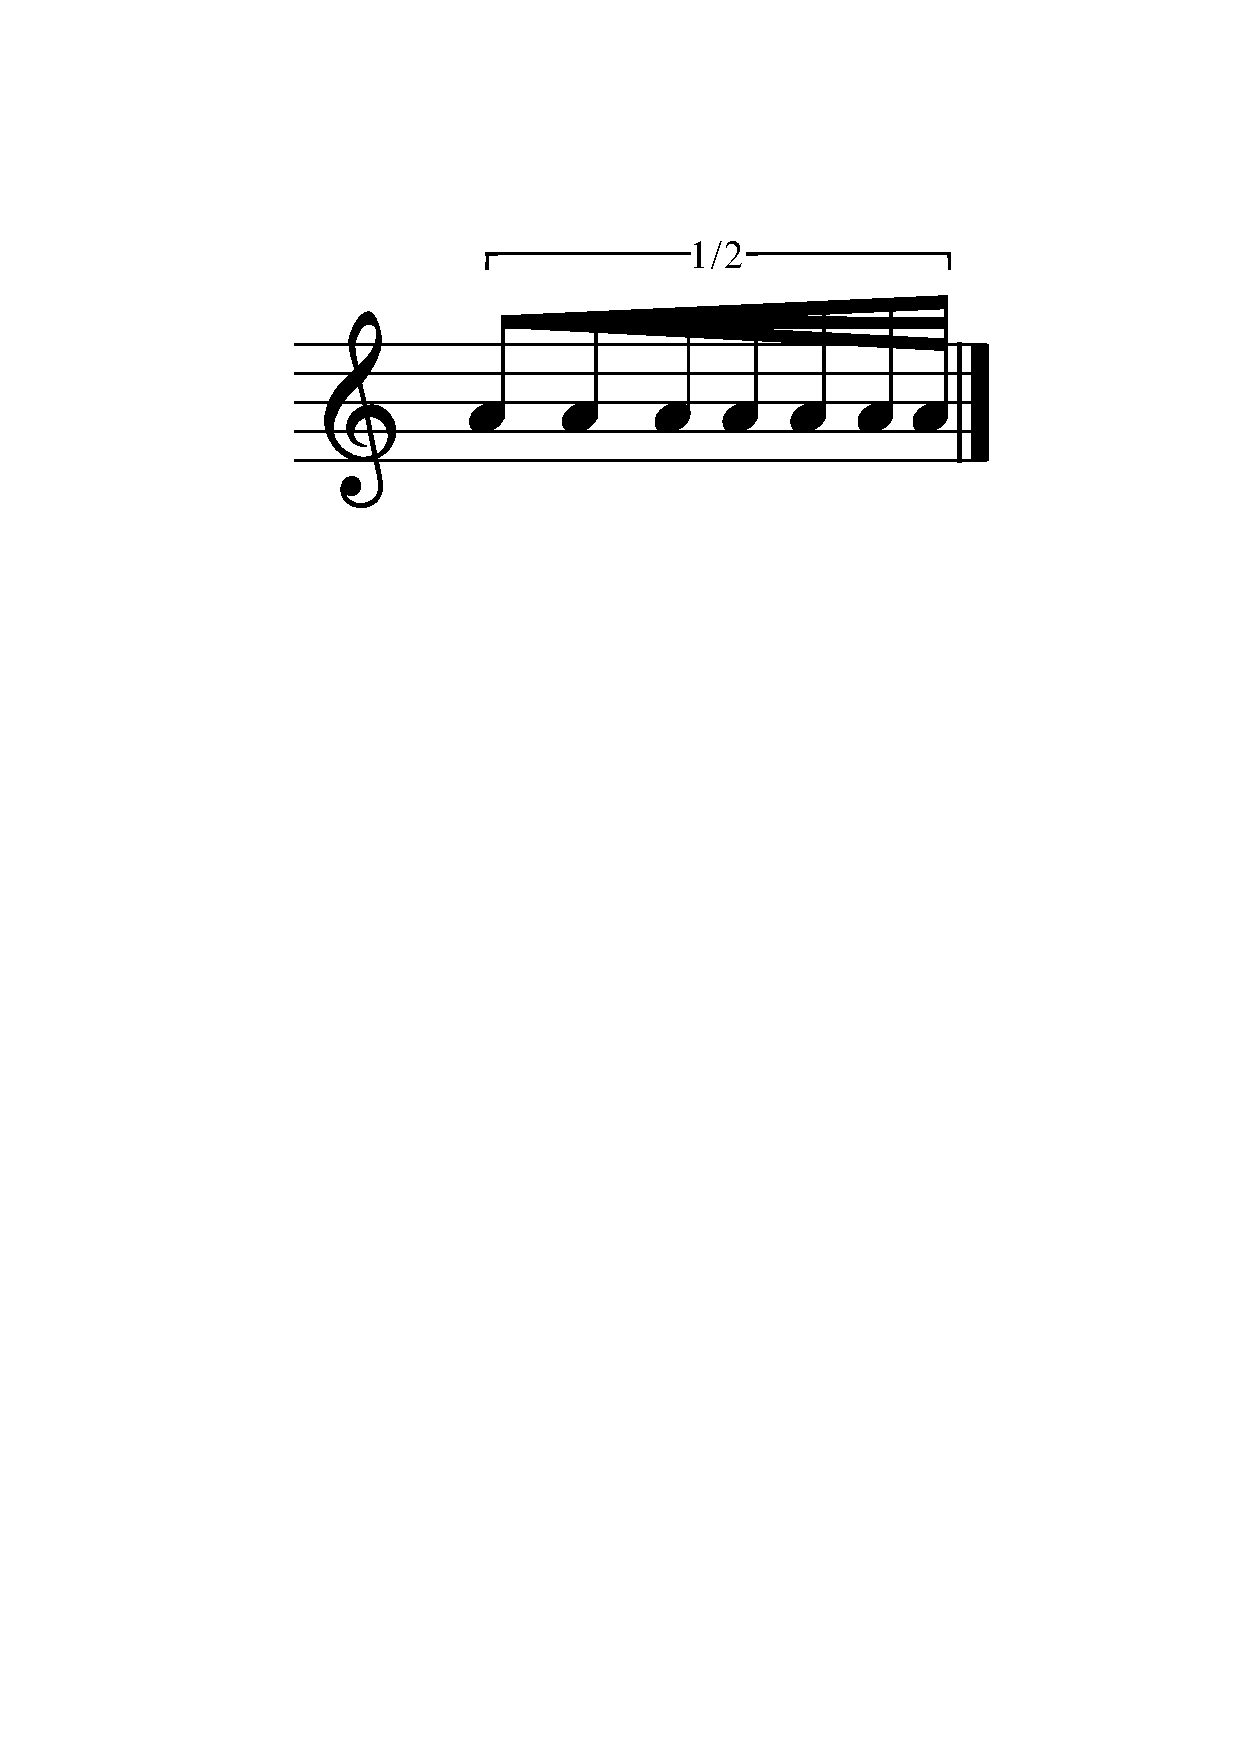
\includegraphics[width=40mm]{img/fbeamduree.pdf}
\caption{Représentation de la durée}
\label{fig:fbeamduree}
\end{figure}

Sans plus d'indication de sa part, l'aspect graphique suivra les durées réelles des notes et prendra comme points de départ et d'arrivée les durées de la première et dernière notes.  C'est le cas de la Figure \ref{fig:fbeamduree}.

En revanche, le paramètre \code{durations} pourra lui permettre d'imposer un aspect graphique tout autre, lui donnant ainsi la possibilité d'indiquer à l'interprète un changement de tempo plus ou moins important, et pas nécessairement cohérent avec les durées intrinsèques des notes, mais ayant du sens dans l'interprétation (Figure \ref{fig:utilisateur}).

%%
\begin{comment}
Ainsi, les deux descriptions suivantes sont valides, mais pas équivalentes :
\\

\begin{figure}[h]
\centering
\begin{gmncode}
[ 
  \fBeam<drawDuration="true">
  (a/16 a a a/32 a/64 a) 
]
\end{gmncode}

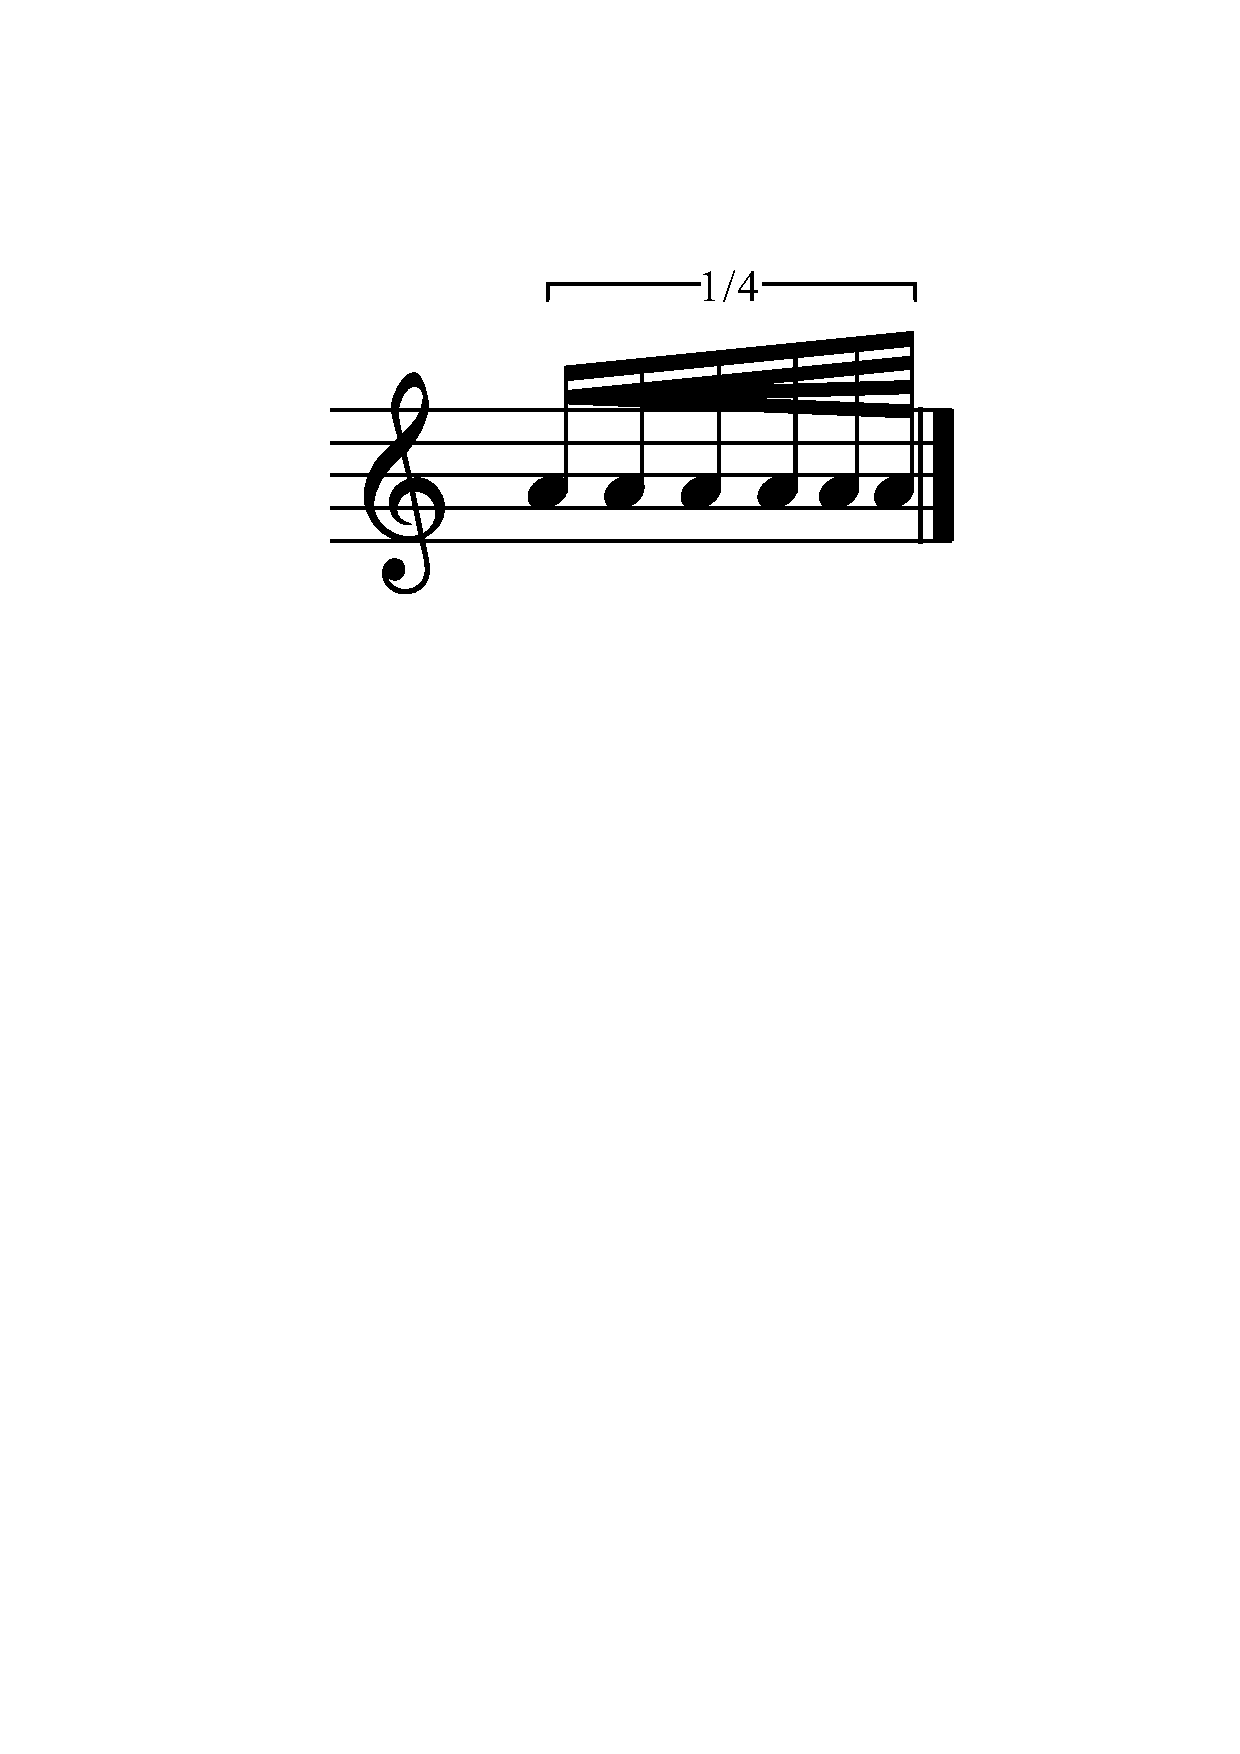
\includegraphics[width=5cm]{img/durationsinternes.pdf}
\caption{Aspect graphique imposé par les durées internes}
\label{fig:interne}
\end{figure}
\end{comment}
%%

\exemple
\begin{figure}[h]
\centering
\begin{gmncode}
[ 
  \fBeam<durations="1/16,1/64", 
  drawDuration="true">
   (a/8 a/16 a a a/32 a) 
]
\end{gmncode}

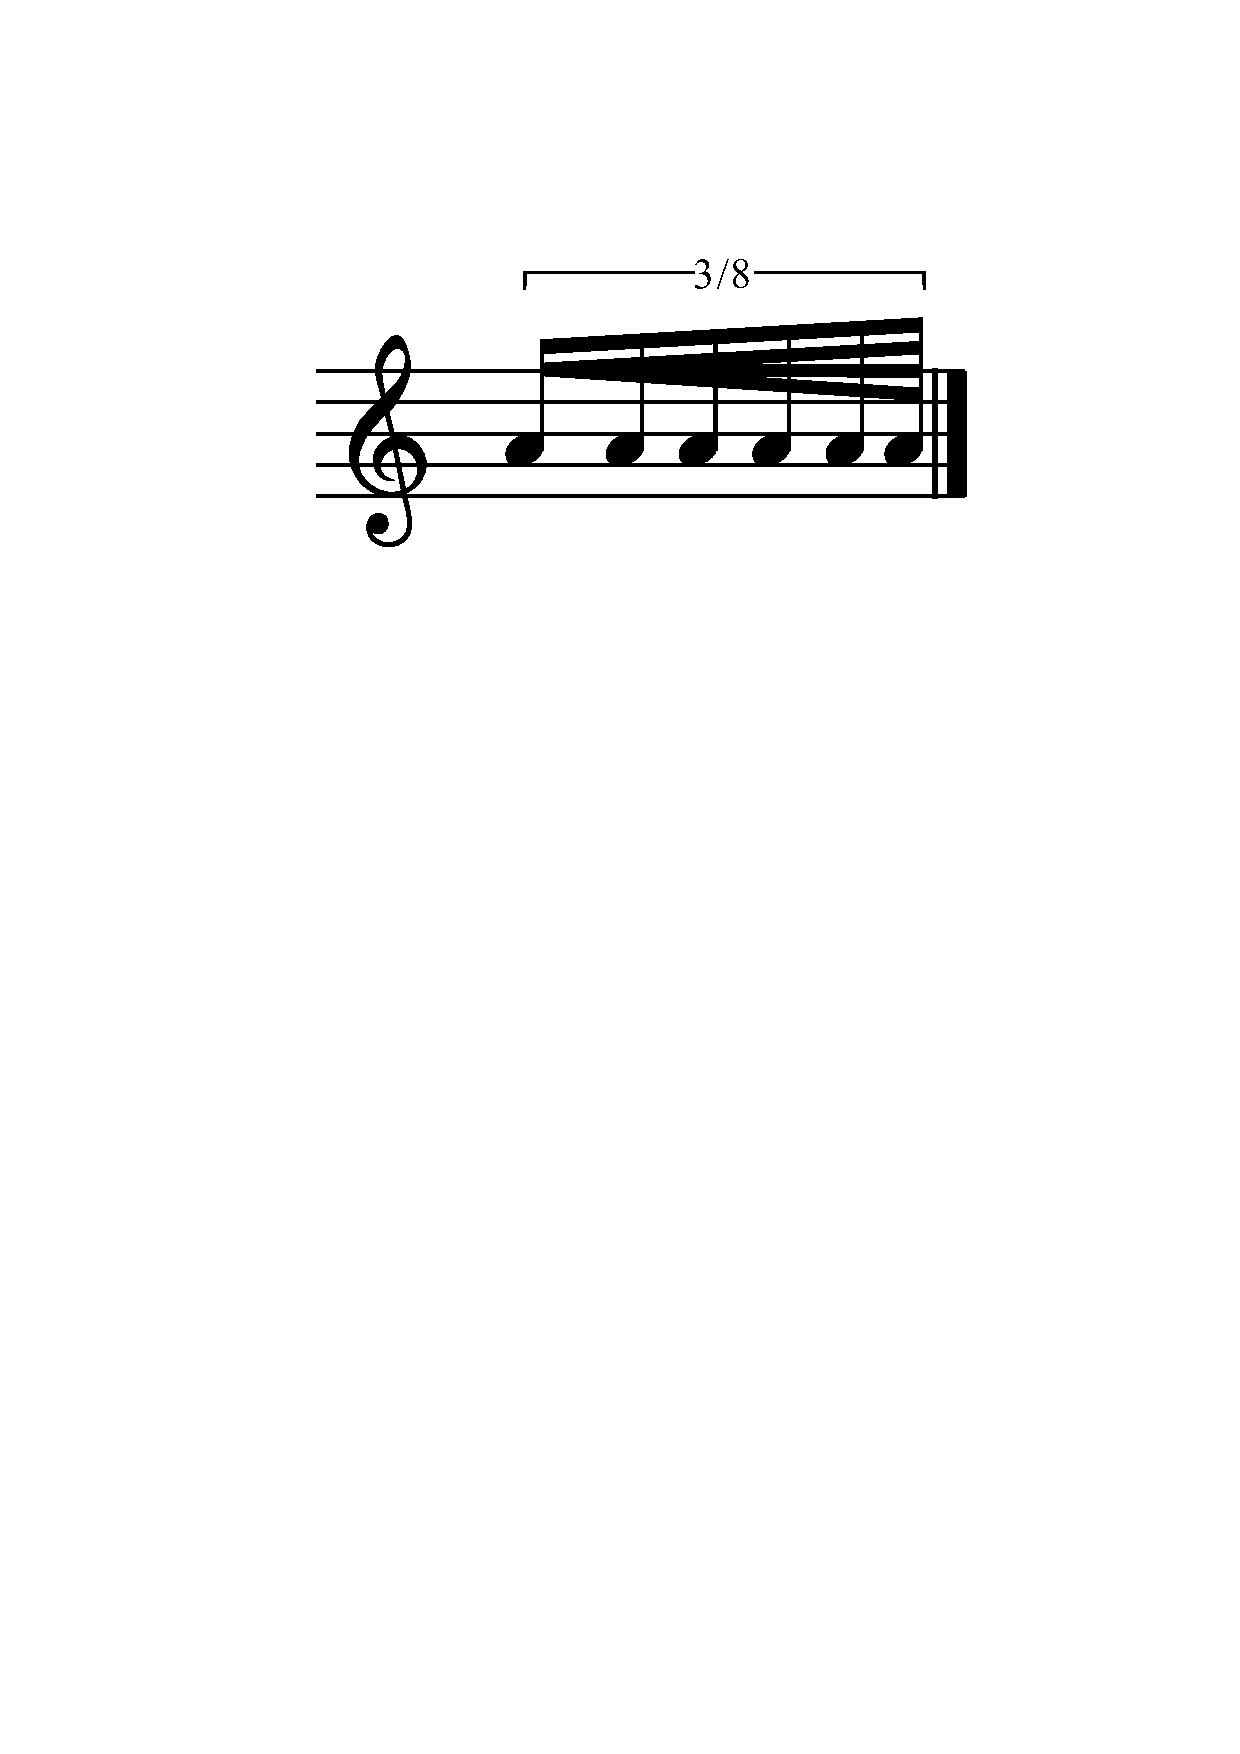
\includegraphics[width=35mm]{img/durations.pdf}
\caption{Aspect graphique imposé par l'utilisateur}
\label{fig:utilisateur}
\end{figure}


% *****************STAFFOFF/ON**********************
\subsection{Tags \textbackslash{}\emph{staffOff} / \textbackslash{}\emph{staffOn}}\label{subsec:staffoff}

\vspace{2mm}
\begin{gmncode}
[ ... \staffOff ... \staffOn ... ]
\end{gmncode}


% littérature ?????????????
% lilypond : même principe, mais les notes et autres éléments se dessinent dans le vide
% permet aussi de passer d'un style de portée à un autre (override staff) ex : 2 lignes...

Les tags \guidotag{staffOff} et \guidotag{staffOn} permettent de faire disparaître et apparaître la partition, en particulier pour cacher une voix muette pendant un certain temps (Figure \ref{fig:staffoffsimple}).

Son usage est généralisé à tous les éléments et toutes les voix de la partition et permet des \emph{montages} plus complexes. (Figure \ref{fig:staffoffexotique})



\begin{figure}[h]
\exemple
\begin{center}
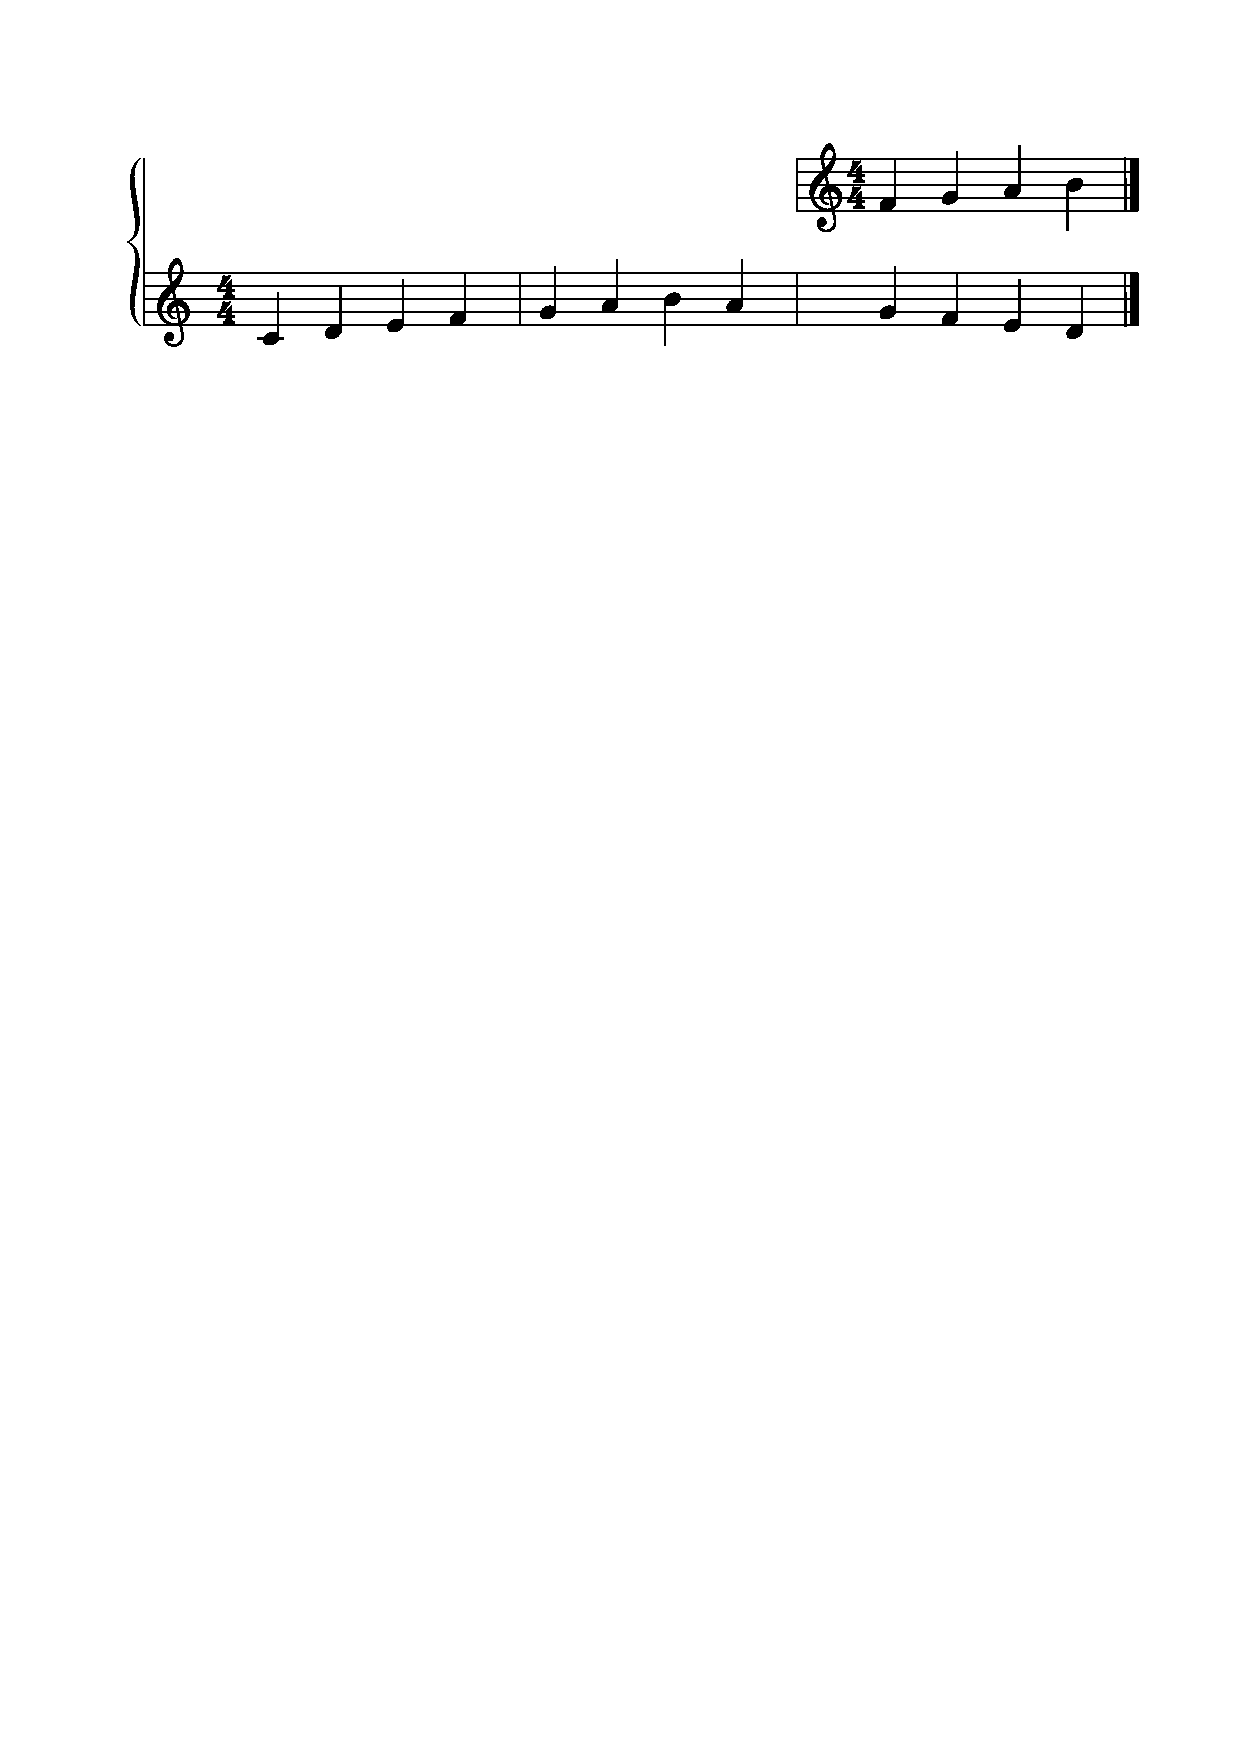
\includegraphics[width=\columnwidth]{img/staffoff.pdf}
\end{center}
\caption{ \guidotag{staffOff} classique}
\label{fig:staffoffsimple}
\end{figure}

%{[\meter<"3/4"> a b/2 c \staffOff g/4 e _\staffOn e a/2 \staffOff \slur(e g) \staffOn a b/4 ], [\meter<"3/4"> \staffOff \clef e \staffOn d g \staffOff _/2 g e g \staffOn a b g d/4]}

\begin{figure}[h]
\centering
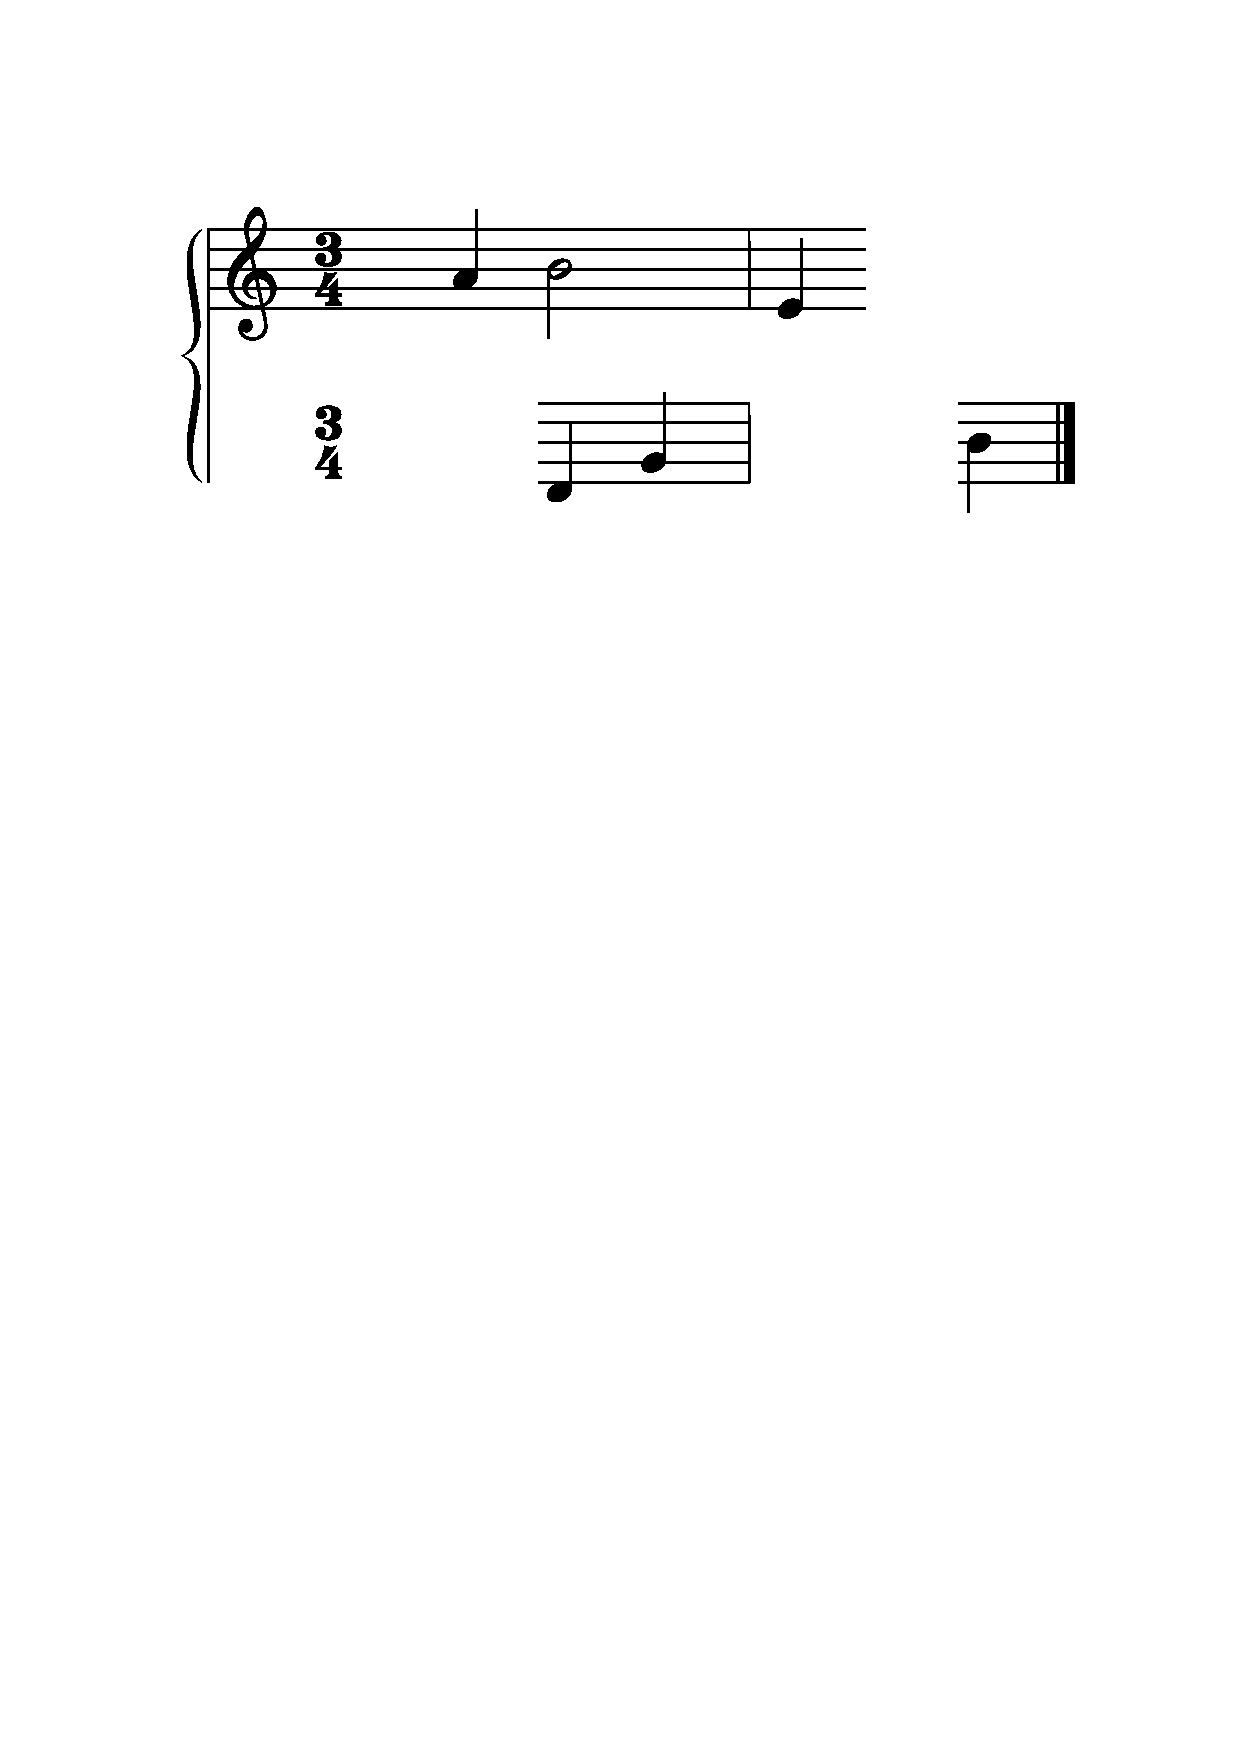
\includegraphics[width=0.8\columnwidth]{img/staffoffexotique.pdf}
\caption{ \guidotag{staffOff} plus complexe}
\label{fig:staffoffexotique}
\end{figure}

L'implémentation graphique est le pendant de la description textuelle : tous les éléments inscrits après un tag \guidotag{staffOff} dans la description textuelle ne sont pas dessinés jusqu'au prochain \guidotag{staffOn} dans la séquence courante. Pour plusieurs éléments simultanés, c'est donc bien l'ordre dans la description textuelle qui indiquera le comportement à adopter. Ainsi, écrire :
\begin{gmncode}
[\meter<"4/4">\clef\staffOff a b\staffOn c]
\end{gmncode}
\vspace{1mm}
n'est pas équivalent à :
\vspace{1mm}
\begin{gmncode}
[\staffOff\meter<"4/4">\clef a b\staffOn c]
\end{gmncode} 

Quant à la portée, elle commence, ou s'arrête, aux positions correspondant au début des éléments suivant le tag.


%************************ GRAPHIQUES ABSTRAITES ******************
\subsection{Graphiques arbitraires}\label{subsec:graphiquesAbstraites}
\bigskip

\begin{gmncode}
1) \symbol<params>
2) \symbol<params>( notes )
  params : 
    - filePath : chemin du fichier
    - position = [top | mid | bot] :
      position de l'image
    - size : taille de l'image
    - w/h : largeur/hauteur de l'image
\end{gmncode}

Le tag \guidotag{symbol} permet d'insérer des graphiques arbitraires dans la partition, sous forme de fichier image externe. Les formats graphiques supportés sont de type \emph{png}, \emph{jpg} ou \emph{bmp}. Les paramètres de contrôle permettent d'ajuster la taille et la position de l'image dans la partition.

Le tag \guidotag{symbol} peut être utilisé comme un tag simple ou comme un range-tag :
\begin{itemize}
	\item 1) le symbole ne possède pas de durée mais prend de place sur la portée, selon sa taille;
	\item 2) le symbole s'applique aux notes indiquées (sans étirement).
\end{itemize}

Pour les deux exemples suivants, les fichiers images sont appelés par un chemin relatif et se situent dans le même répertoire que le fichier \gmn{} (contenant le code de l'exemple) ouvert.

\exemple\\
Le code suivant produit le résultat présenté en figure \ref{fig:symbol}. Sur la première portée, le symbole ne possède pas de durée, contrairement à la deuxième portée.

\begin{gmncode}
{
  [
    \meter<"4/4"> c f
  \symbol<file="silence.png",dx=-5,dy=-10> 
    c d f
  ],
  [
    \meter<"4/4"> a d
  \symbol<file="ronds.png",position="bot"> 
  (f g) g
  ]
}
\end{gmncode}

\begin{figure}[h]
\centering
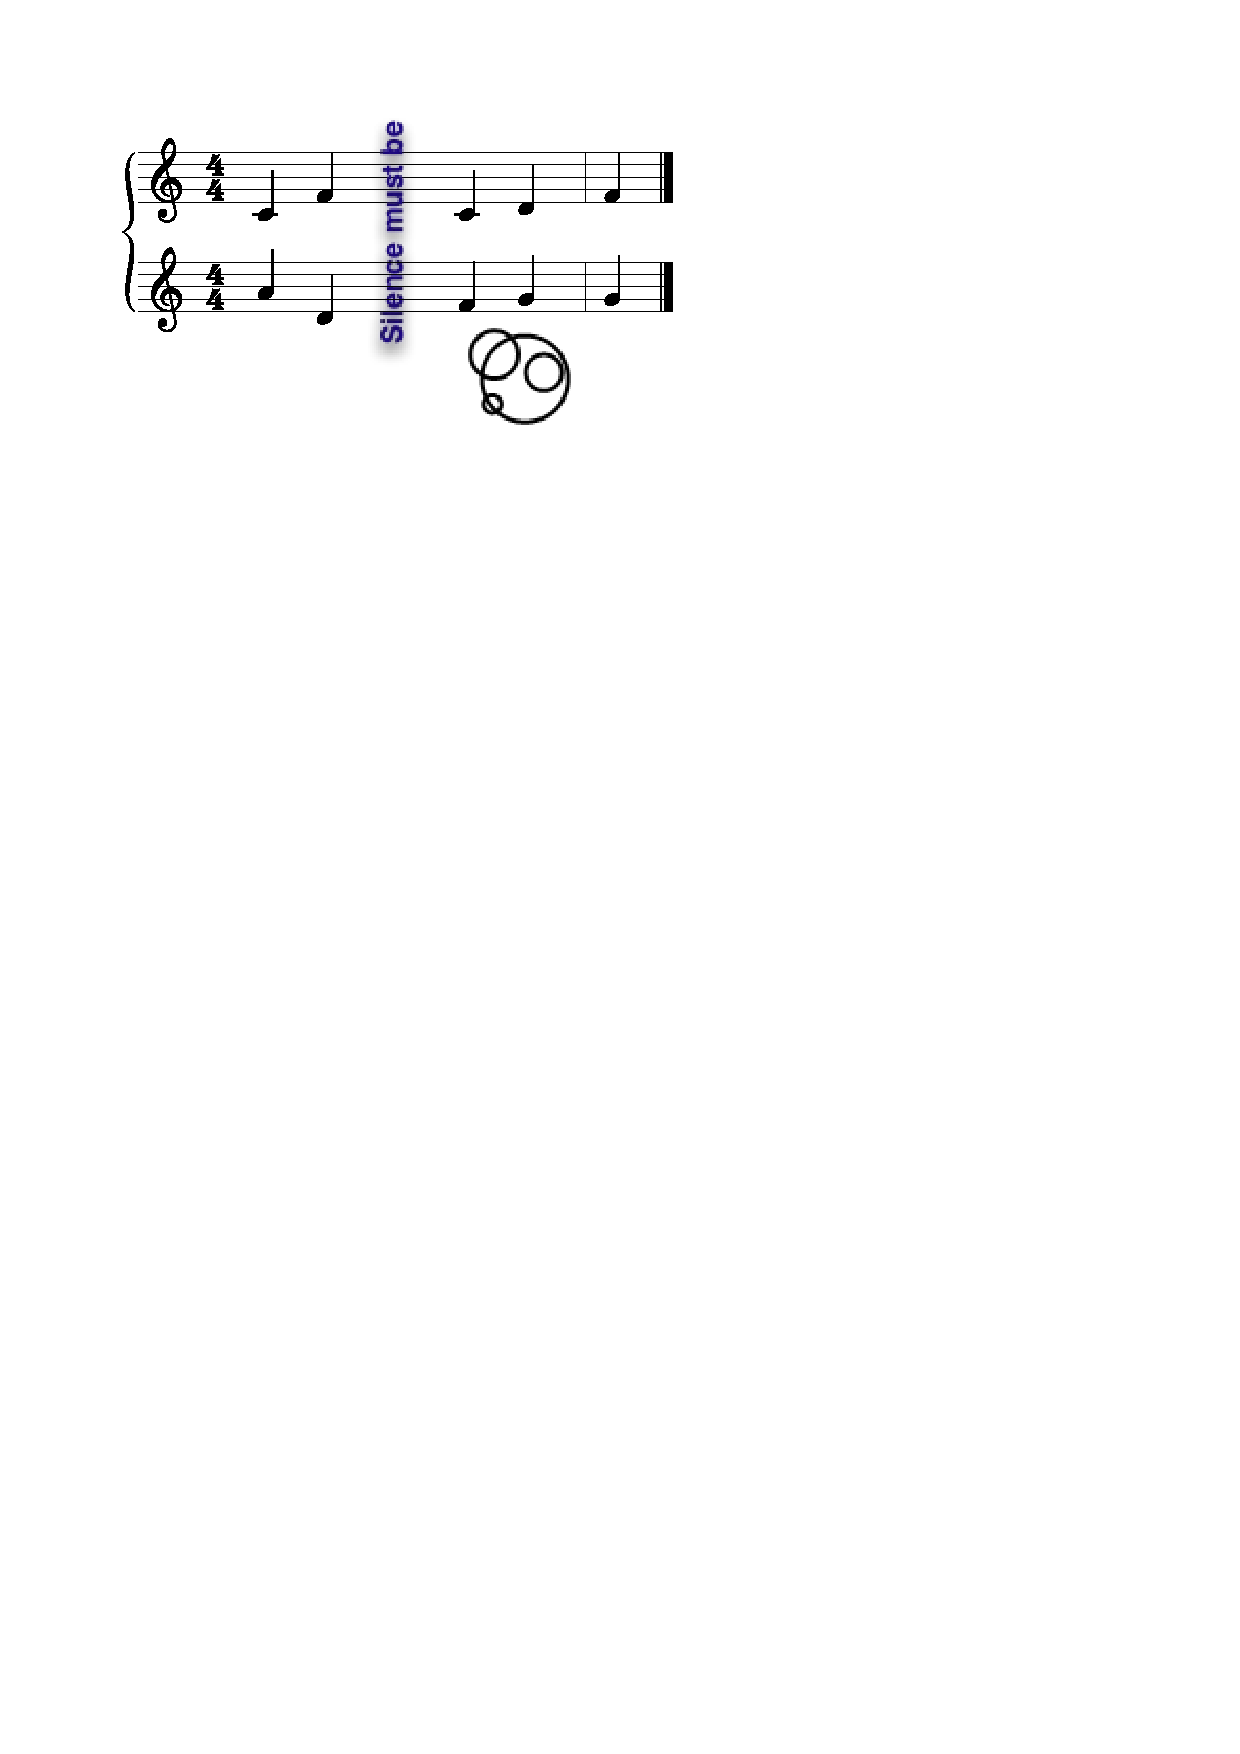
\includegraphics[width=65mm]{img/partitions/symbol.pdf}
\caption{Graphiques arbitraires}
\label{fig:symbol}
\end{figure}

Le fichier est indiqué par un chemin absolu ou relatif. Dans le second cas, le chemin est relatif au répertoire contenant le fichier source ou au répertoire \emph{home} de l'utilisateur.

Divers paramètres spécifiques permettent de contrôler le rendu graphique :
\begin{itemize}
	\item \code{position} (\code{top}, \code{mid} ou \code{bot}), position de l'image par rapport à la portée;
	\item \code{size}, contrôle de la taille;
	\item \code{w/h}, réglage de la largeur et/ou de la hauteur de l'image;
\end{itemize}

%************************ AMELIORATIONS DIVERSES ******************
\subsection{Améliorations diverses}\label{subsec:amelioraions}


%*****************TRILLES********************
\subsubsection{Trilles}\label{subsubsec:trilles}

% littérature
% lilypond : e\trill f\trill ... sans vaguelette sinon \startTrillSpan ... \stopTrillSpan
%\gardner Read

\begin{gmncode}
  \trill<params>(chord-series)
   params:
    - tr = [true | false]
    - anchor = [note | tr]
\end{gmncode}

% Citation wiki
Un \emph{trille} est \og{}un ornement musical qui consiste à alterner très rapidement la note de base (la note principale), sur laquelle est noté le \emph{trille}, et la note située juste au-dessus\fg{}.

Dans la version précédente de \guido{}, le \emph{trille} à proprement parler n'était indiqué que par le symbole \textit{\textbf{tr}} placé au dessus de la note. Il paraissait pourtant important que la notation comprenne également la ligne ondulée du \emph{trille} qui suit celui-ci et en indique la durée. Comme ce symbole était déjà en partie implémenté, il fallait pouvoir lui offrir plus de souplesse sans pour autant en complexifier la notation.

%D'après Elaine Gould \cite{gould2011behind}, la ligne du \emph{trille} doit être dessinée depuis le signe \textit{\textbf{tr}} jusqu'au début du prochain évènement (la prochaine note ou le prochain soupir), sauf si celui-ci se situe directement après la prochaine barre de mesure, la ligne s'arrêtant dans ce cas à la barre elle-même. 

% justifier l'intérêt de tr et anchor ?
De plus, nous avons voulu donner la possibilité de choisir de dessiner ou non le signe \textit{\textbf{tr}}, ainsi que de pouvoir changer l'ancrage de la ligne pour le déplacer sur la tête de la note. Cela fut implémenté grâce au \emph{param} \code{tr} qui accepte comme valeurs \code{true} ou \code{false} et \code{anchor} qui accepte comme valeurs \code{note} ou \code{tr} (Figure \ref{fig:trillanchor}). Le reste des modifications graphiques pouvant être effectuées manuellement par l'utilisateur à travers les paramètres classiques de déplacement (\code{dx}, \code{dy}), de couleur (\code{color}), et de taille (\code{size}).

\exemple
\begin{figure}[h]
\centering
\begin{gmncode}
[ \trill<tr="false", anchor="note">
( {g} {a/2} ) ]
\end{gmncode}
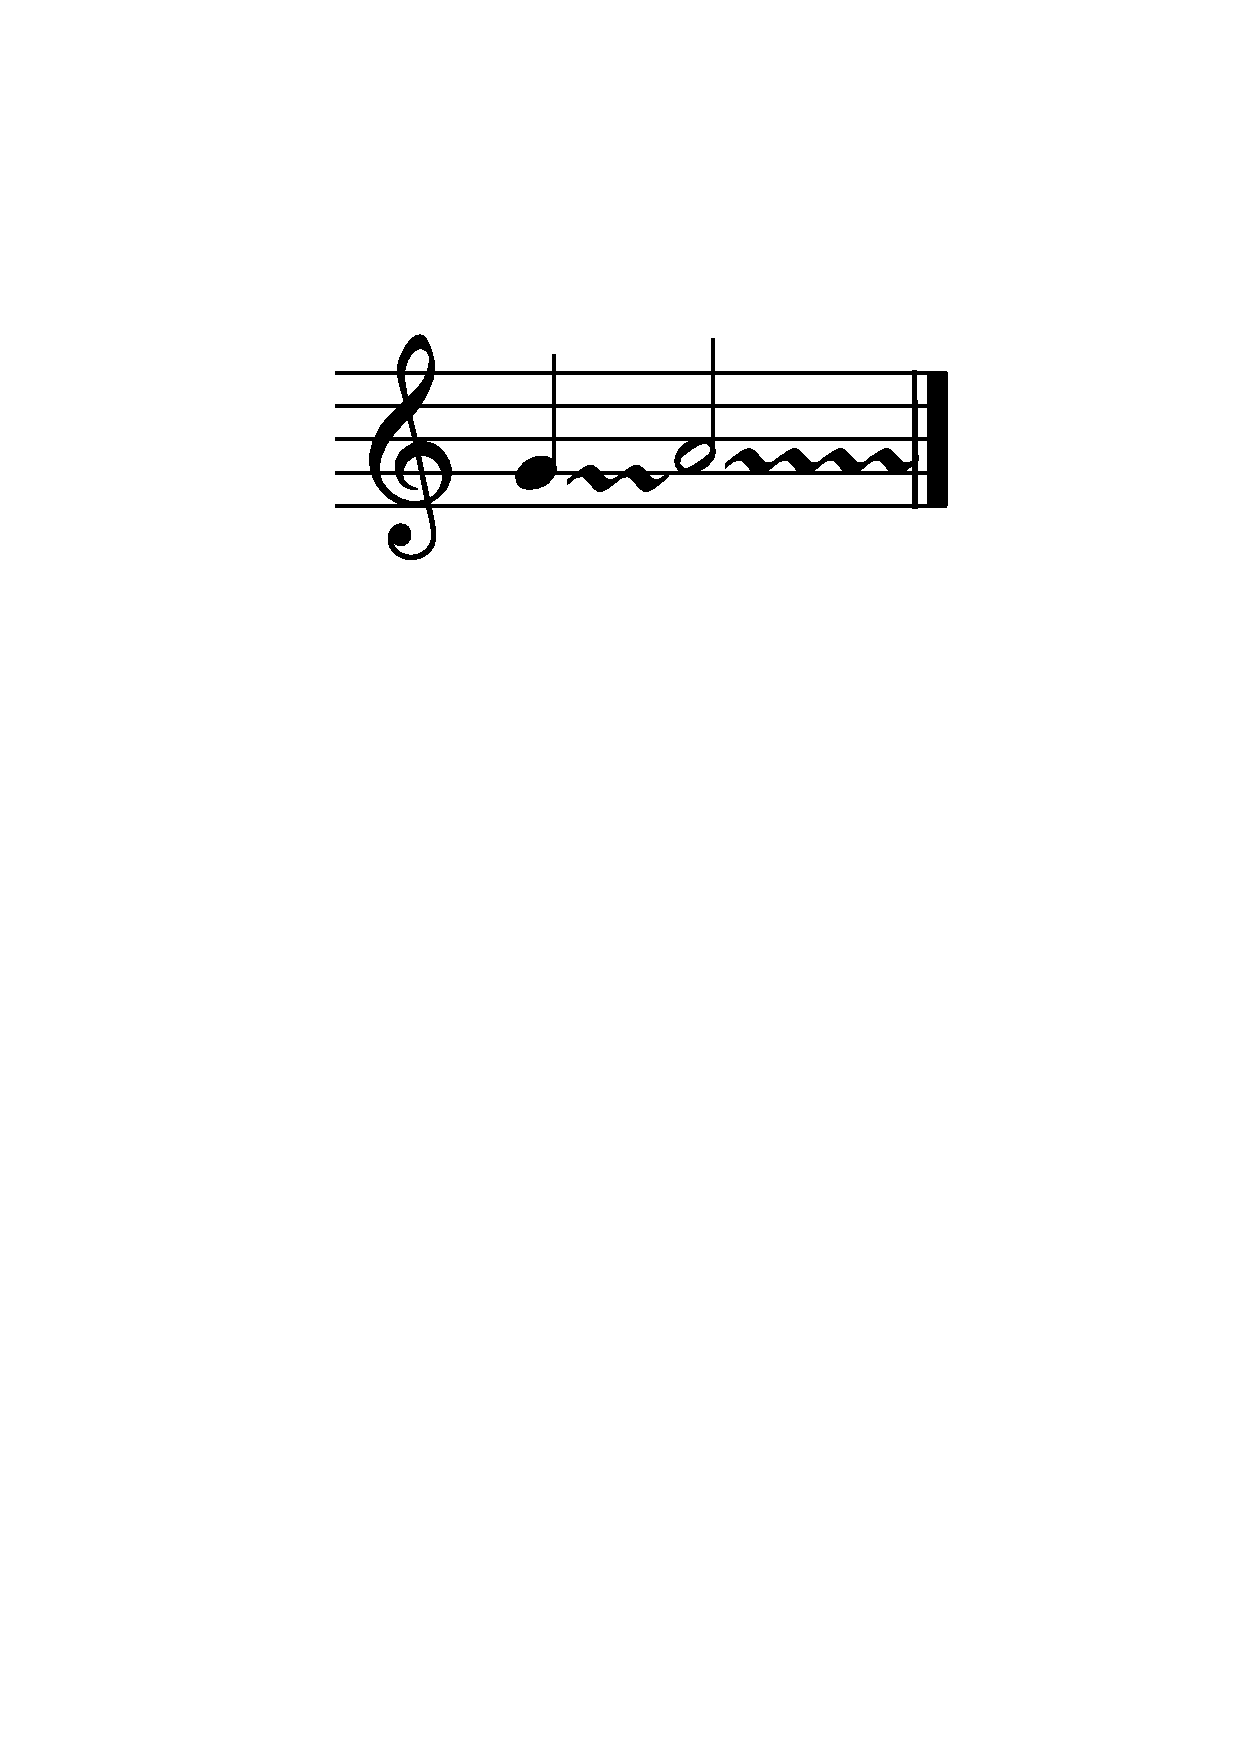
\includegraphics[width=30mm]{img/trillanchor.pdf}
\caption{Cas du \emph{trille} ancré à la tête de note, et \textit{\textbf{tr}} optionnel}
\label{fig:trillanchor}
\end{figure}

%************************* NOUVEAUX ATTRIBUTS **************************
\subsubsection{Nouveaux attributs}\label{subsubsec:attributs}

Le tag \guidotag{accol} permet de paramétrer l'accolade liant les portées d'une partition. Depuis la version 1.52, celle-ci peut changer de style et posséder un \emph{range}, c'est-à-dire qu'elle n'est plus obligée d'englober toute la partie musicale. De plus, plusieurs accolades peuvent être affichées en même temps. L'exemple de la figure \ref{fig:accol} illustre ceci.

\begin{figure}[h]
\centering
\begin{gmncode}
{
  [
    \accol<id=1, range="1-3",
      dx=-4, type="straightBrace"> a b c
  ],
  [
    \accol<id=2, range="1-2">
    \clef<"f"> c0/2
  ],
  [
    c d e
  ]
}
\end{gmncode}
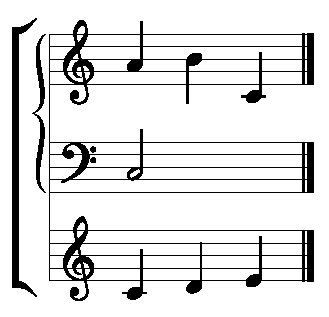
\includegraphics[width=40mm]{img/partitions/accol.pdf}
\caption{Nouveaux paramétrages de l'accolade}
\label{fig:accol}
\end{figure}

\bigskip

Dans \guido{}, la direction du \emph{marcato} ne pouvait auparavant pas être choisie par l'utilisateur, ceci a été modifié (cf. figure \ref{fig:marcato}).

\begin{figure}[h]
\centering
\begin{gmncode}
[
  \marcato(a)
  \marcato<"above", dy=4> (a)
]
\end{gmncode}
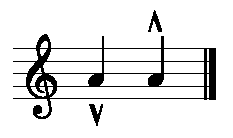
\includegraphics[width=30mm]{img/partitions/marcato.pdf}
\caption{Orientation forcée du \emph{marcato}}
\label{fig:marcato}
\end{figure}

\bigskip

Le tag \guidotag{staffFormat} s'est également vu doter d'un nouveau paramètre, \code{lineThickness}, permettant de gérer l'épaisseur des lignes de la portée (cf. \ref{fig:lineThickness}).

\begin{figure}[h]
\centering
\begin{gmncode}
[
  \staffFormat<lineThickness=0.5>  c d e f 
]
\end{gmncode}
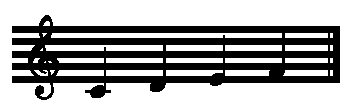
\includegraphics[width=40mm]{img/partitions/staffFormat.pdf}
\caption{Tag \guidotag{staffFormat} : nouveau \emph{param}}
\label{fig:lineThickness}
\end{figure}

\bigskip

Nous avons rajouté trois nouveaux \emph{params} au tag\\ \guidotag{tuplet} (cf. figure \ref{fig:tuplet}) :
\begin{gmncode}
1) lineThickness :
   épaisseur des lignes latérales
2) bold = [true | false] :
   style typographique de la valeur du tuplet
3) textSize : 
   taille de la valeur du tuplet
\end{gmncode}

\begin{figure}[h]
\centering
\begin{gmncode}
[
  \tuplet<"-3-", lineThickness=0.4,
    bold="true", textSize=2, dy1=10>
  (a a a)
]
\end{gmncode}
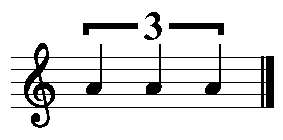
\includegraphics[width=35mm]{img/partitions/tuplet.pdf}
\caption{Tag \guidotag{tuplet} : nouveaux \emph{params}}
\label{fig:tuplet}
\end{figure}

\bigskip

Dans les versions précédentes de \guido{}, le crescendo/ decrescendo n'était pas personnalisable, ceci a été amélioré dans la version 1.52 (cf. figure \ref{fig:crescDecresc}). Sept nouveaux \emph{params} ont vu le jour :
\begin{gmncode}
1) dm = [pp | p | f | ff ...] :
intensité du crescendo/decrescendo
2) dx1 :
offset horizontal de la gauche du symbole
3) dx2 :
offset horizontal de la droite du symbole
4) dy :
offset vertical du symbole
5) deltaY :
écartement des deux droites du symbole
6) color :
couleur du symbole
7) size :
taille du marqueur d'intensité
\end{gmncode}

\begin{figure}[h]
\centering
\begin{gmncode}
{
  [
    \cresc<dm="ff", dx1=2, dx2=-4, dy=1,
      deltaY=5, color="red", size=2>
    (a b e)
  ],
  [
    \decresc<thickness=0.5> (a f/2 f/4)
  ]
}
\end{gmncode}
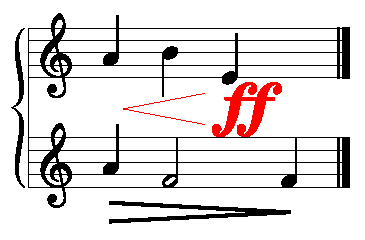
\includegraphics[width=40mm]{img/partitions/crescDecresc.pdf}
\caption{Tag \guidotag{cresc} et \guidotag{decresc} : nouveaux \emph{params}}
\label{fig:crescDecresc}
\end{figure}

%%%%%%%%%%%%%%%%%%%% CONTROLE DE RENDU %%%%%%%%%%%%%%%%%
\section{Contr\^ole de rendu}\label{sec:controleRendu}

%*************************GLISSANDI ET ACCORDS*******************************
\subsection{Glissandi et accords}\label{subsec:glissandiAccords}

Un \emph{glissando} entre deux accords soulève la question la répartition des \emph{glissandi} entre les notes des accords. La solution proposée est celle qui nous a paru la plus intuitive : c'est l'ordre des notes dans la description textuelle de l'accord qui détermine les relations entre les notes, c'est à dire : pour 2 accords A t B, la première note de l'accord A sera liée à la première note de l'accord B, la seconde de A à la seconde de B, etc.(Figure \ref{fig:glissandosimple})


\begin{figure}[h]
\exemple
\begin{center}
\begin{gmncode}
[\glissando({e,a} {f,b} {a,d})]
\end{gmncode}
\bigskip

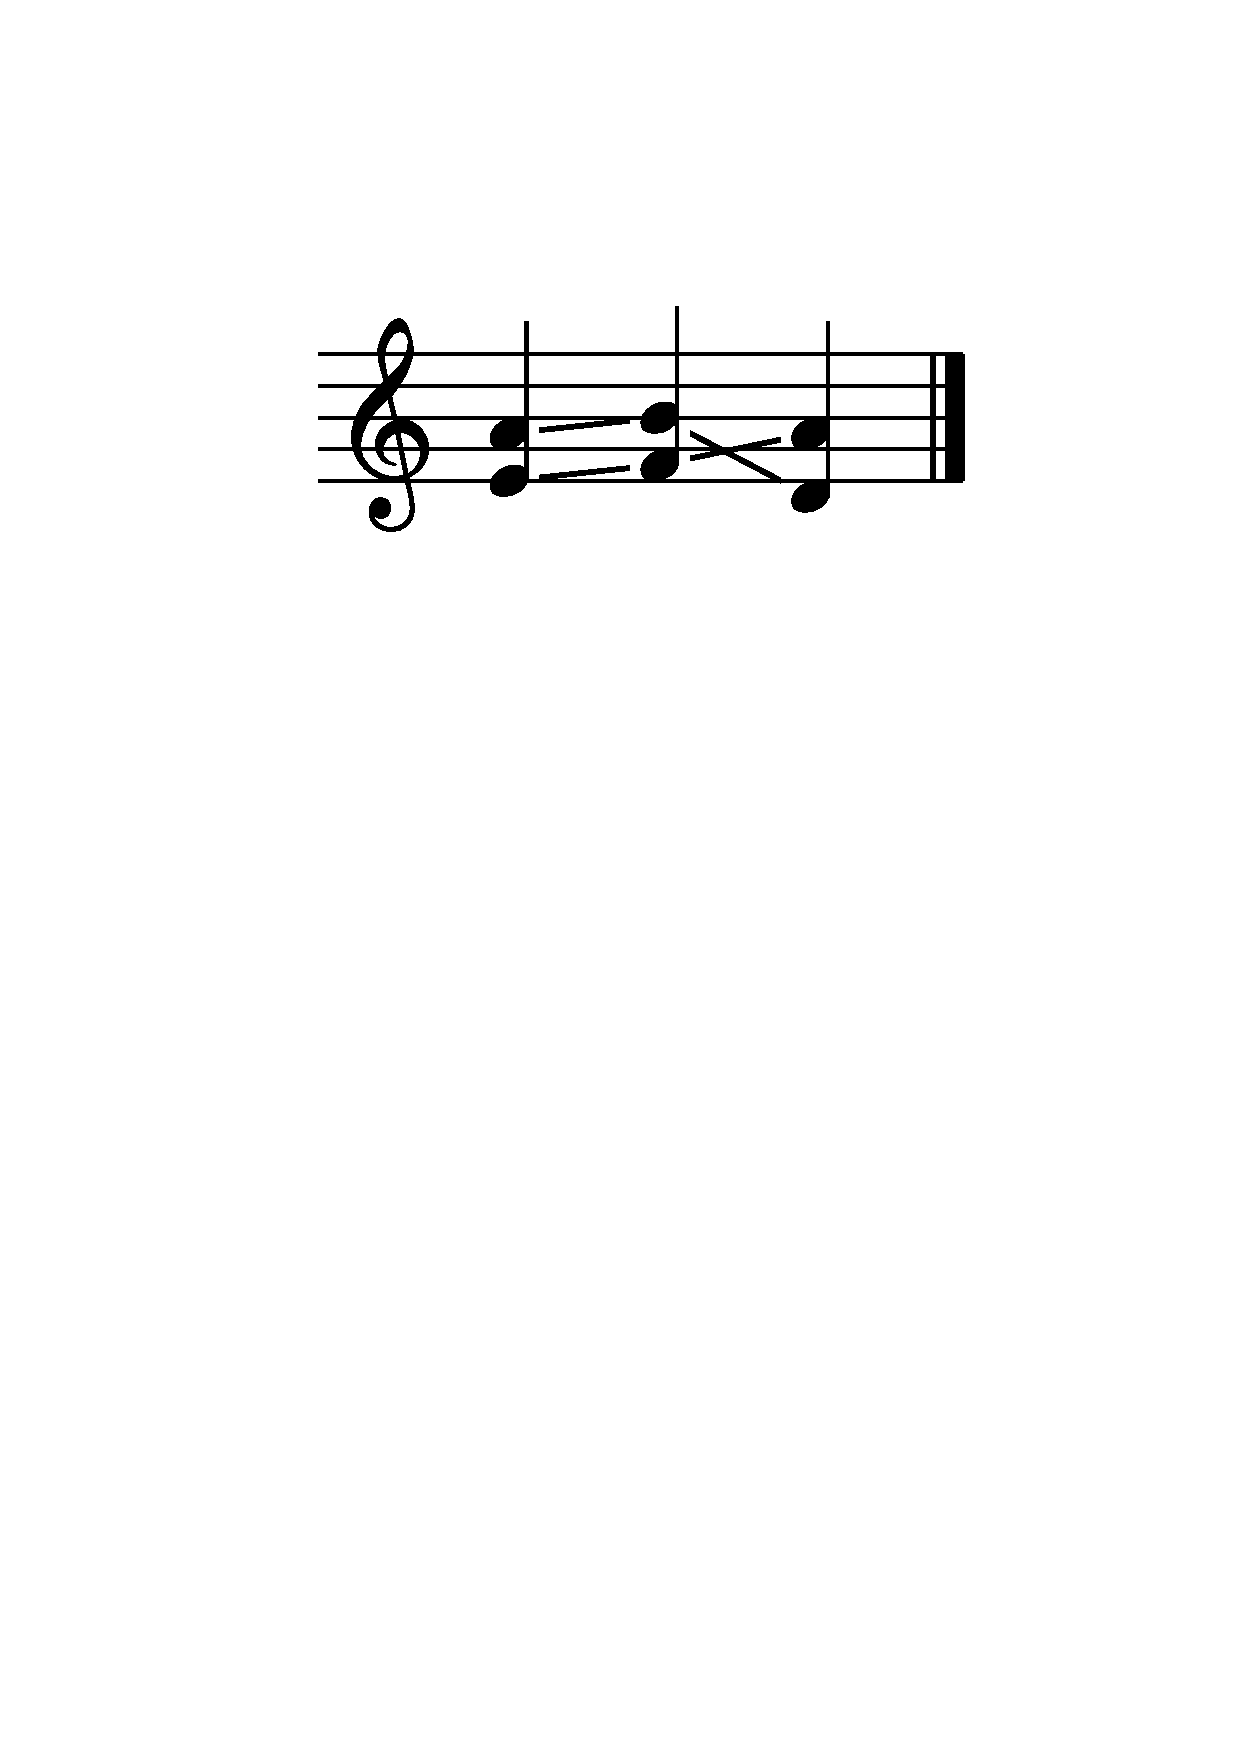
\includegraphics[width=35mm]{img/glissandosimple.pdf}
\caption{\emph{glissandi} entre accords}
\label{fig:glissandosimple}
\end{center}
\end{figure}

L'unique problème avec ce choix peut se poser lors d'un conflit dans l'ordre imposé par le glissando précédent et par le suivant, comme dans le premier cas de l'exemple Figure \ref{fig:glissandopb}. Il est alors possible de faire appel à une seconde voix, et au tag \guidotag{staff\textless{}numero de portée\textgreater{}} qui pourra créer sur une même portée d'autres glissandi en parallèle et indépendants des premiers (Figure \ref{fig:glissandopb}).

\exemple
\begin{figure}[h]
\centering
\begin{gmncode}
[ \glissando(e {d,f,a} g) b ]
\end{gmncode}
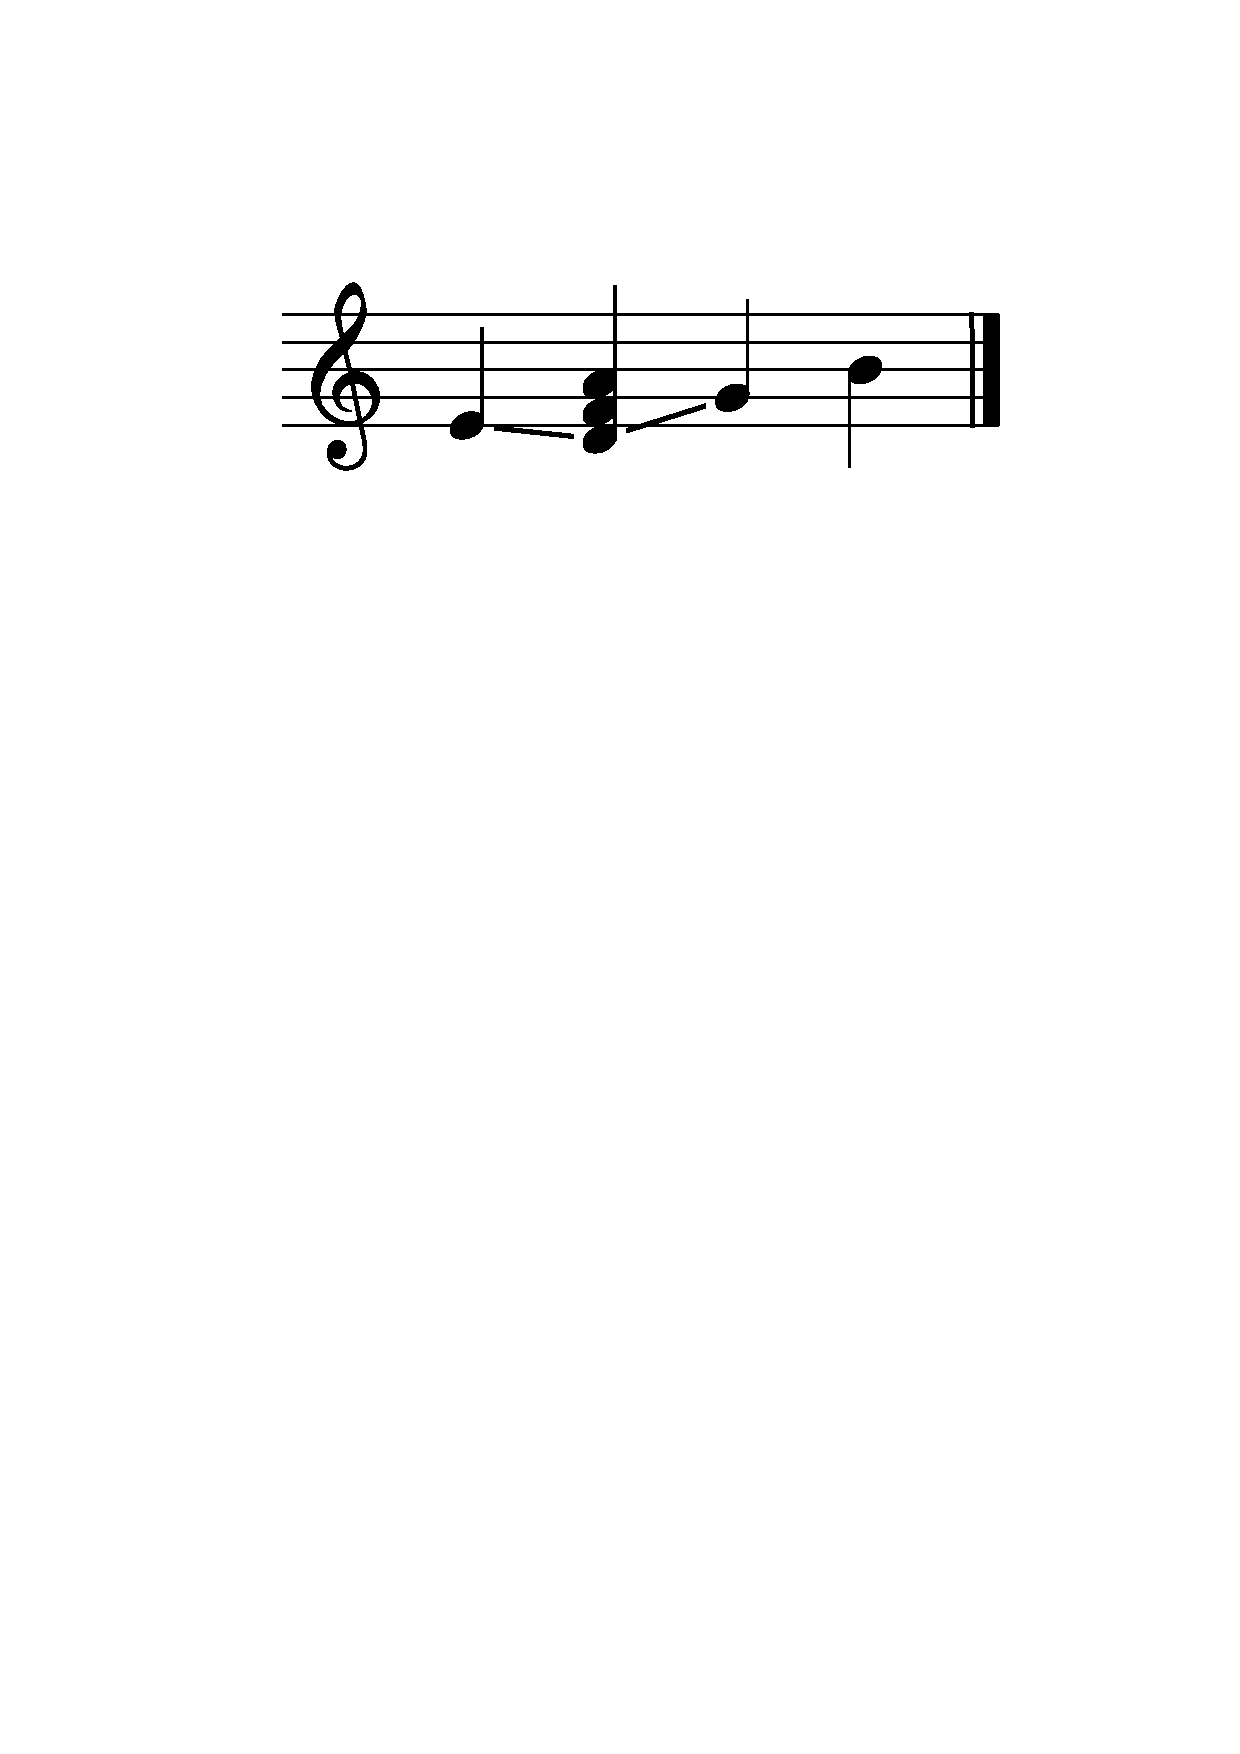
\includegraphics[width=4cm]{img/glissandopb.pdf}

\begin{gmncode}
{ 
  [ \glissando( e {d,f}) empty b ],
  [ \staff<1> empty \glissando( a g ) empty ] 
}
\end{gmncode}
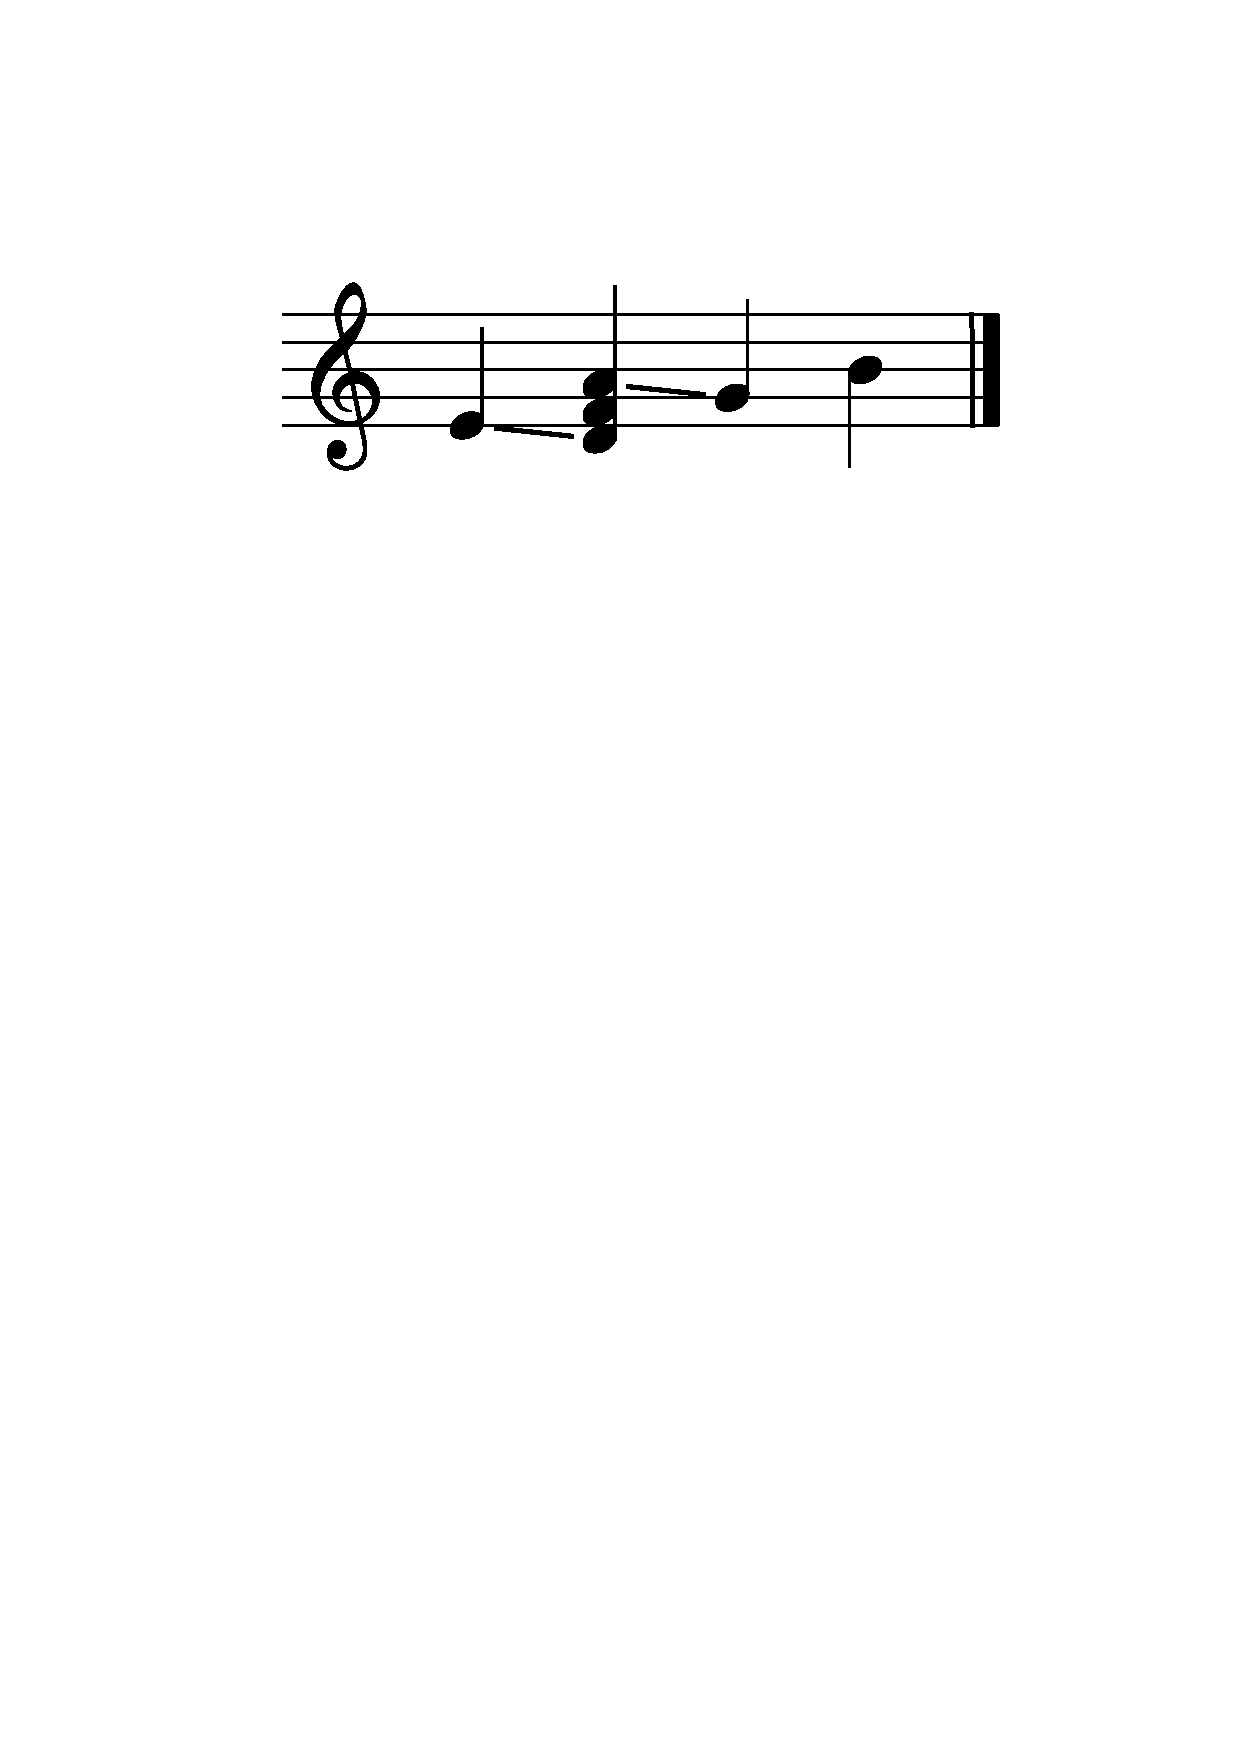
\includegraphics[width=4cm]{img/glissandosanspb.pdf}
\caption{Cas de recours à une seconde voix pour le \emph{glissando} -
\code{empty} représente une note vide.}
\label{fig:glissandopb}
\end{figure}


%*****************************TRILLES ET TIES****************************************
\subsection{Trilles et liaisons}\label{subsec:trillesLiaison}

Au niveau du trille, une subtilité au niveau du contr\^ole du rendu a également été ajoutée. Il fallait définir le comportement quant aux notes liées, soit de manière automatique de par la présence d'une barre de mesure, soit de manière explicitement décrite par l'utilisateur. La solution adoptée est de dessiner la ligne de \emph{trille} jusqu'à la fin de la dernière note liée si celle-ci provient d'une note plus longue découpée automatiquement, mais de s'arrêter normalement à la prochaine note si la liaison a été explicitée par l'utilisateur, qui pourra alors décider de répéter le \emph{trille} sur cette autre note, ou non. (Figure \ref{fig:trill})

\exemple
\begin{figure}[h]
\centering
\begin{gmncode}
{
  [\meter<"2/4"> \trill({a} {a/2})],
  [\meter<"2/4"> \trill({a} \tie({a} {a}))]
}
\end{gmncode}
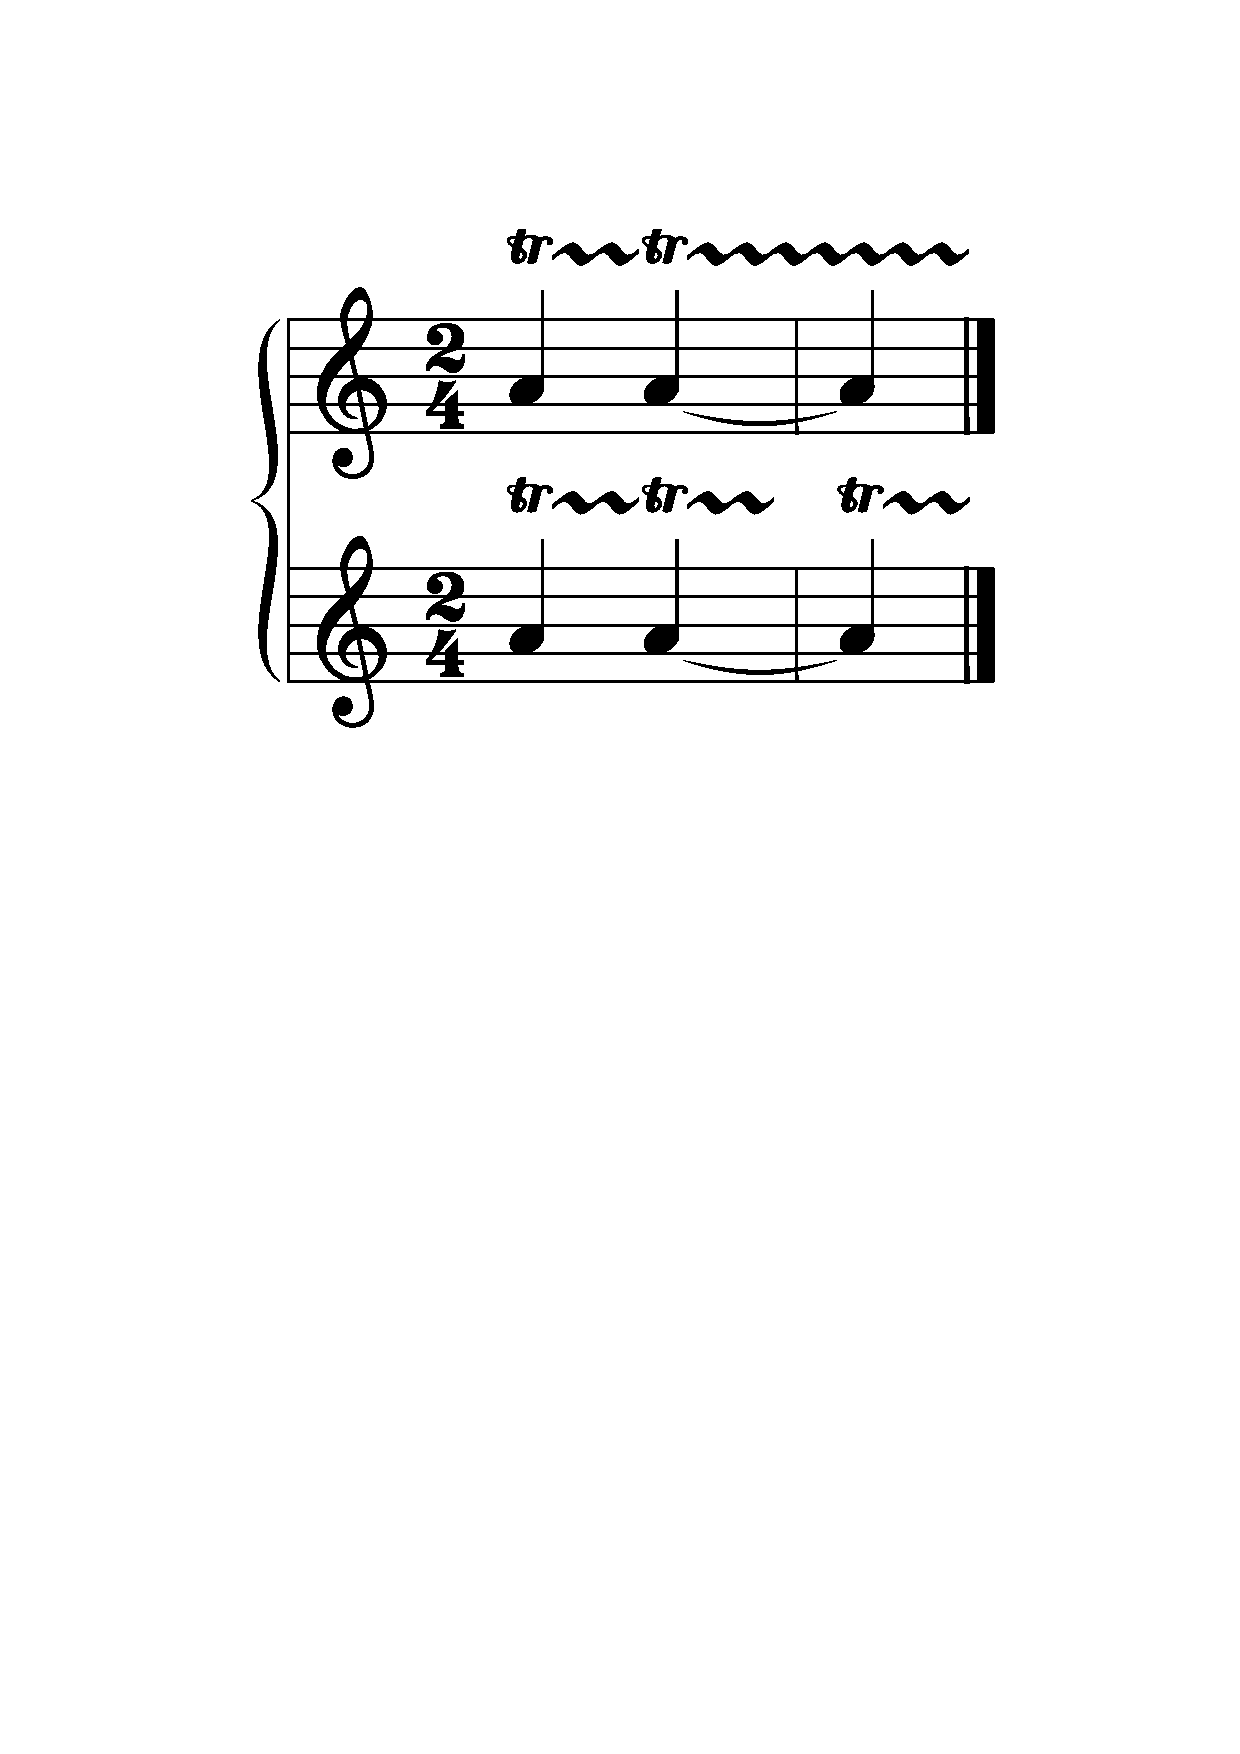
\includegraphics[width=45mm]{img/trill.pdf}
\caption{Cas du \emph{trille} appliqué à des notes liées}
\label{fig:trill}
\end{figure}

%%%%%%%%%%%%%%%%%%%% COMBINAISONS %%%%%%%%%%%%%%%%%
\section{Combinaisons}\label{sec:combinaisons}

%*****************************GLISSANDI ET CLUSTERS****************************************
\subsection{\emph{Glissandi} et \emph{clusters}}\label{subsec:glissandiCluster}

Lors de combinaisons de \emph{glissandi}  avec des accords ou des \emph{clusters}, il nous a paru intéressant, comme on peut le voir dans \cite{gould2011behind} (p.143) ou dans \cite{stone1980music} (p.61), de donner la possibilité de remplir l'espace entre ces \emph{glissandi} grâce à un \emph{param} \code{fill}. Une certaine flexibilité peut être trouvée dans le dessin grâce aux \emph{params} graphiques \code{dx1}, \code{dx2}, \code{dy1}, \code{dy2}, ainsi que \code{thickness} qui permettent de modifier l'aspect du \emph{glissando}. (Figure \ref{fig:glissandofill})

\exemple
\begin{figure}[h]
\begin{center}
\begin{gmncode}
[ 
  \glissando<fill="true", dx1=-2, dx2=2, 
   thickness=2.2>(\cluster({e,g} {c,b}))
  \glissando<fill="true">({c,e,g} {a,c2,f1}) 
]
\end{gmncode}

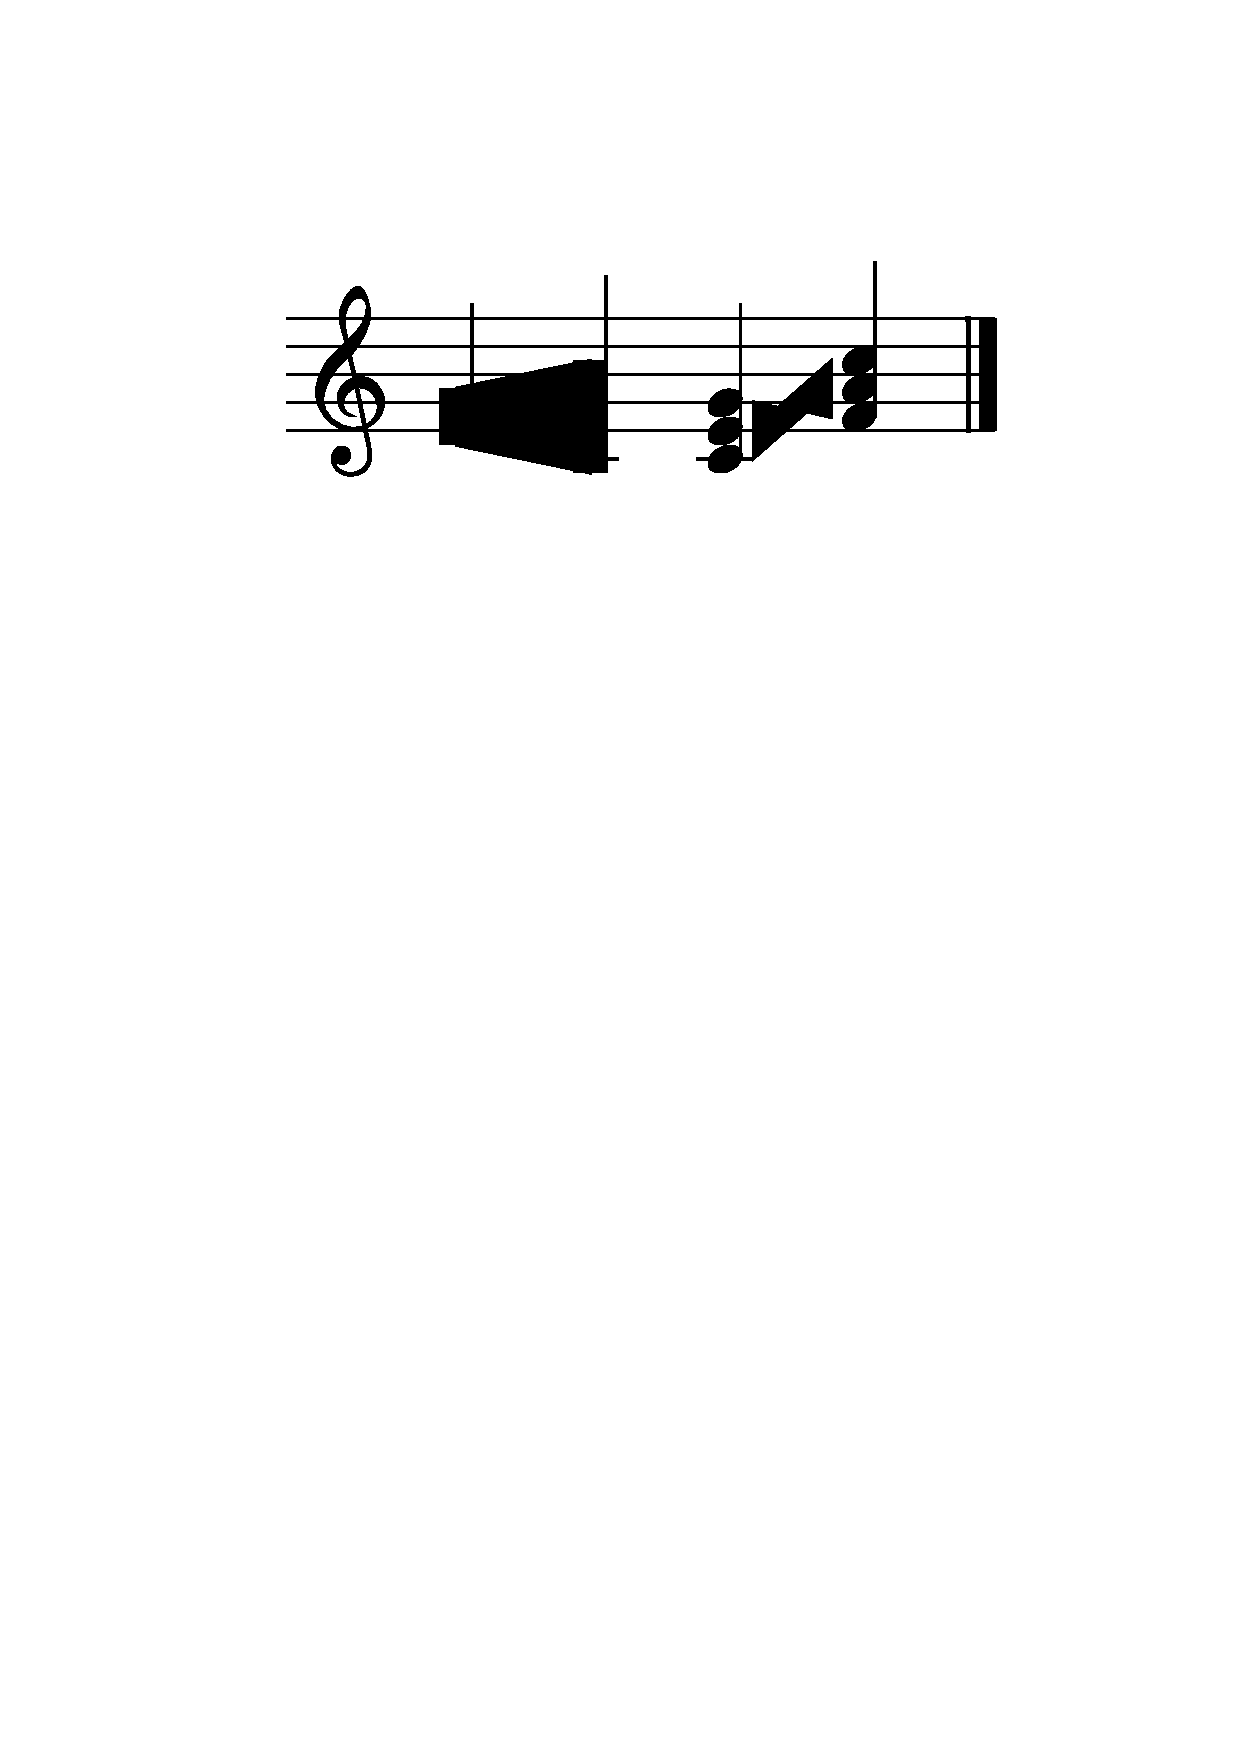
\includegraphics[width=4cm]{img/glissandofill.pdf}
\caption{\emph{glissandi} entre accords et clusters avec \emph{param} de remplissage}
\label{fig:glissandofill}
\end{center}
\end{figure}

%*****************************HIERARCHIE BEAMS****************************************
\subsection{Combinaisons de \emph{beams}}\label{subsec:combinaisonBeams}

% justification des hierarchies de beams ?
Enfin, concernant le \emph{feathered beam} comme le \emph{beam} classique, il est maintenant possible de créer des hierarchies de \emph{beams} : c'est à dire d'englober plusieurs \emph{beams} dans un plus grand, afin de les joindre par une barre principale commune (Figure \ref{fig:fbeamhierarchie}).

\exemple
\begin{figure}[h]
\centering
\begin{gmncode}
[ 
  \beam( 
    \fBeam(c/8 e d f g/32) 
    \fBeam(a/16 f e d c/64) 
  ) 
]
\end{gmncode}

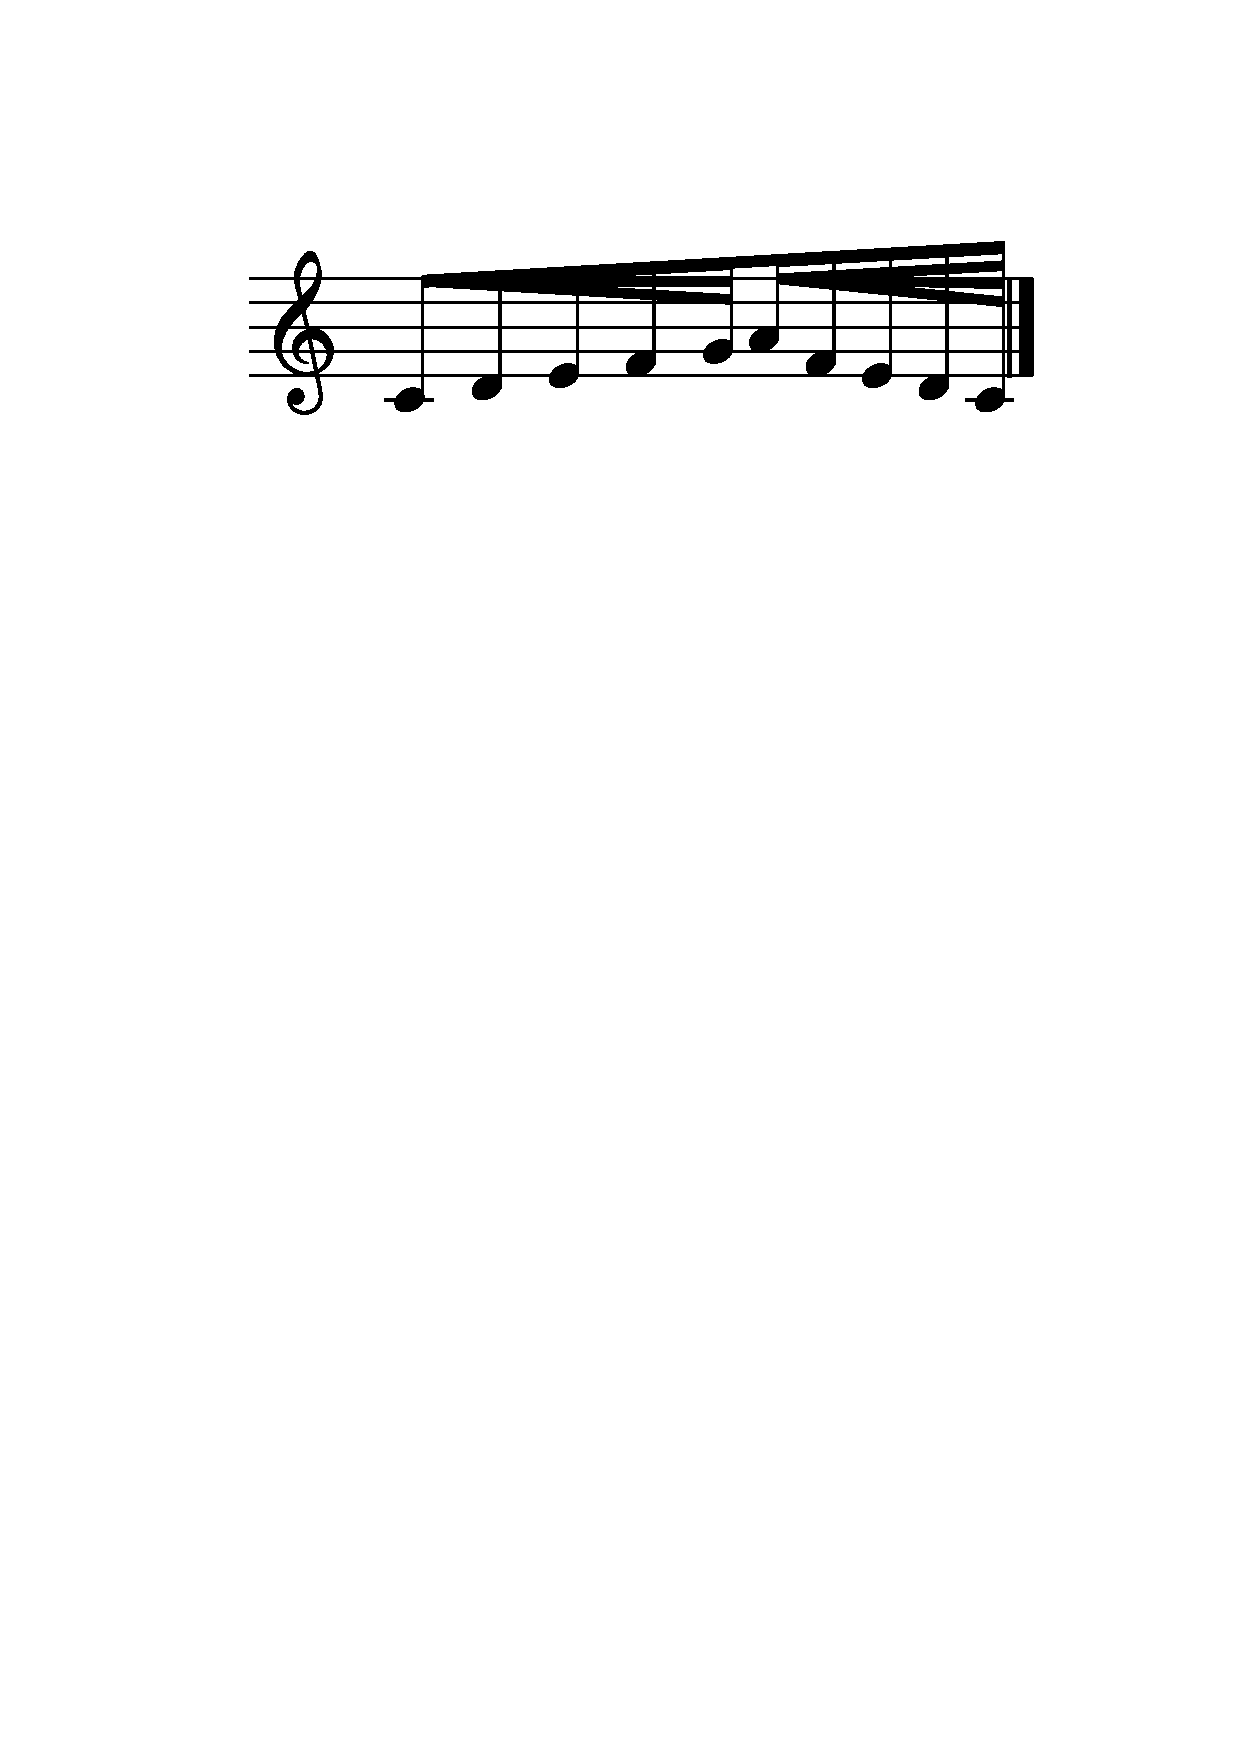
\includegraphics[width=55mm]{img/fBeamHierarchie.pdf}
\caption{\emph{Feathered beams} englobés dans un plus grand}
\label{fig:fbeamhierarchie}
\end{figure}


%*********************CONCLUSION**********************
\section{Conclusion}\label{sec:conclusion}
Les extensions présentées dans cet article ont été réalisées principalement à la demande de compositeurs et au service de créations en cours. Elles s'intègrent dans le moteur existant dans le respect des différentes combinaisons du langage. Leur implémentation a soulevé des problèmes de design qui ont été résolus en laissant à l'utilisateur le choix entre les différentes possibilités. Elles sont disponibles avec la version 1.52 de la librairie \guido{}.


\balance
\bibliographystyle{plain}
\bibliography{../../guido}


\end{document}

